\documentclass[twoside,11pt]{article}

% Any additional packages needed should be included after jmlr2e.
% Note that jmlr2e.sty includes epsfig, amssymb, natbib and graphicx,
% and defines many common macros, such as 'proof' and 'example'.
%
% It also sets the bibliographystyle to plainnat; for more information on
% natbib citation styles, see the natbib documentation, a copy of which
% is archived at http://www.jmlr.org/format/natbib.pdf

\usepackage{jmlr2e}
\usepackage{booktabs}
\usepackage{amsmath}
\usepackage{tikz}
\usepackage[font=small,format=hang]{caption}
\usepackage{subcaption}
\usepackage{fontawesome}
\usepackage{ifthen}
\usepackage{xstring}
\usepackage{pgfopts}
\usepackage{tikz-uml}
% \usepackage{algorithm2e}
\usepackage{algorithm}
\usepackage[noend]{algpseudocode}

\usetikzlibrary{positioning, backgrounds, decorations.pathreplacing, arrows, arrows.meta, calc}

% Definitions of handy macros can go here

% \def\faPython{\symbol{"F3E2}}


\newcommand{\dataset}{{\cal D}}
\newcommand{\fracpartial}[2]{\frac{\partial #1}{\partial  #2}}

% Heading arguments are {volume}{year}{pages}{submitted}{published}{author-full-names}

% \jmlrheading{1}{2000}{1-48}{4/00}{10/00}{Marina Meil\u{a} and Michael I. Jordan}

% Short headings should be running head and authors last names

\ShortHeadings{Learning to reinforcement learn for Neural Architecture Search}{J. Gomez Robles}
\firstpageno{1}

\begin{document}

\title{Learning to reinforcement learn for Neural Architecture Search\thanks{MSc thesis supervised by dr. ir. Joaquin Vanschoren at the Eindhoven University of Technology}}


\author{\name Jorge Gomez Robles \email j.gomez.robles@student.tue.nl \\
       \addr Department of Mathematics and Computer Science\\
       Eindhoven University of Technology\\
       Eindhoven 5612 AZ, The Netherlands
}

% \editor{Joaquin Vanschoren}

\maketitle

\begin{abstract}%   <- trailing '%' for backward compatibility of .sty file
This is an abstract. This is an abstract. This is an abstract. This is an abstract. This is an abstract. This is an abstract. This is an abstract. This is an abstract. This is an abstract. This is an abstract. This is an abstract. This is an abstract. This is an abstract. This is an abstract. This is an abstract. This is an abstract. This is an abstract. This is an abstract. This is an abstract. This is an abstract. This is an abstract. This is an abstract. This is an abstract. This is an abstract. This is an abstract. This is an abstract. This is an abstract. This is an abstract. This is an abstract. This is an abstract. This is an abstract. This is an abstract. This is an abstract. This is an abstract. This is an abstract. This is an abstract. This is an abstract. This is an abstract. This is an abstract. This is an abstract. This is an abstract. This is an abstract. This is an abstract. This is an abstract. This is an abstract. This is an abstract. This is an abstract. This is an abstract. This is an abstract. This is an abstract. This is an abstract. This is an abstract. This is an abstract. This is an abstract. This is an abstract. This is an abstract. This is an abstract. This is an abstract. This is an abstract. This is an abstract. This is an abstract. This is an abstract. This is an abstract. This is an abstract. This is an abstract. This is an abstract. This is an abstract. This is an abstract. This is an abstract. This is an abstract. This is an abstract. This is an abstract. 
\end{abstract}

\begin{keywords}
  Neural Architecture Search, Deep Meta-Reinforcement Learning, Image Classification
\end{keywords}

%Todo: check difference between citep and citet
\section{Introduction}

Neural networks have achieved remarkable results in many fields, such as that of Image Classification. Crucial aspects of this success are the choice of the neural architecture and the chosen hyperparameters for the particular dataset of interest; however, this is not always straightforward. Although state-of-the-art neural networks can inspire the design of other architectures, this process heavily relies on the designer's level of expertise, making it a challenging and cumbersome task that is prone to deliver underperforming networks.

In an attempt to overcome these flaws, researchers have explored various techniques under the name of Neural Architecture Search (NAS)~\citep{NASsurvey}. In NAS, the ultimate goal is to come up with an algorithm that takes any arbitrary dataset as input and outputs a well-performing neural network for some learning task of interest, so that we can accelerate the design process and remove the dependency on human intervention. Nevertheless, coming up with a solution of this kind is a complicated endeavor where researchers have to deal with several aspects such as the type of the networks that they consider, the scope of the automation process, or the search strategy applied. A particular search strategy for NAS is reinforcement learning (RL), where a so-called \textit{agent} learns how to design neural networks by sampling architectures and using their numeric performance on a specific dataset as the reward signals that guide the search. Popular standard RL algorithms such as \textsc{Q-learning} or \textsc{Reinforce} have been used to design state-of-the-art Convolutional Neural Networks (CNNs) for classification tasks on the CIFAR and ImageNet datasets \citep{ENAS, PathNAS, BlockQNN, ZophNAS1, BakerNAS}, but little attention is paid to deliver architectures for other datasets. In an attempt to fill that gap, a suitable alternative is deep meta-RL~\citep{LtRL, RL2}, where the \textit{agent} acts on various environments to learn an \textit{adaptive} policy that can be transferred to new environments.

In this work, we apply deep meta-RL to NAS, which, to the best of our knowledge, is a novel contribution. The environments that we consider are associated with standard image classification tasks on datasets with different levels of hardness sampled from a meta-dataset~\citep{MetaDataset}. Our main experiments focus on the design of chain-structured networks and show that, under resource constraints, the resulting policy can adapt to new environments, outperform standard RL, and design better architectures than the ones inspired by state-of-the-art networks. We also experiment with extending our approach to the design of multi-branch architectures so that we can give directions for future work.


The remainder of this report is structured as follows. First, in  Section ~\ref{sec:preliminaries}, we introduce the preliminary concepts required to understand our work. Next, in Section~\ref{sec:related}, we discuss the related work for both reinforcement learning and NAS. In Section~\ref{sec:methodology}, we formally introduce our methodology, and in Section~\ref{sec:software}, the framework developed to implement it. In Section~\ref{sec:experiments}, we define the experiments, and in Section~\ref{sec:results}, we show the results. Finally, in Section~\ref{sec:conclusions}, the conclusions are set out.
\section{Preliminaries}\label{sec:preliminaries}

\subsection{Reinforcement learning}\label{sec:preliminaries:rl}

Reinforcement learning (RL) is an approach to automate goal-directed learning~\citep{RLIntroBook}. It relies on two entities that interact with each other: an \textit{environment} that delivers information of its \textit{state}, and an \textit{agent} that using such information learns how to achieve a \textit{goal} in the environment. The interaction is a bilateral communication where the \text{agent} performs \textit{actions} to modify the \textit{state} of the environment, which responds with a numeric \textit{reward} measuring how good the action was to achieve the \textit{goal}. Typically, the sole interest of the agent is to improve its decision-making strategy, known as the \textit{policy}, to maximize the total reward received over the whole interaction trial since this will lead it to the desired goal. More strictly, RL is formalized using finite Markov Decision Processes (MDPs) as in Definition~\ref{def:preliminaries:rl} borrowed from~\cite{RL2}, resulting in the agent-environment interaction illustrated in Figure~\ref{fig:preliminaries:rl}.


\begin{definition}[Reinforcement Learning]
\label{def:preliminaries:rl}
We define a discrete-time finite-horizon discounted MDP $M = (\mathcal{X}, \mathcal{A}, \mathcal{P}, r, \rho_0, \gamma, T)$, in which $\mathcal{X}$ is a state set, $\mathcal{A}$ an action set, $\mathcal{P}: \mathcal{X} \times \mathcal{A} \times \mathcal{X} \mapsto \mathbb{R}_+$ a transition probability distribution, $r: \mathcal{X} \times \mathcal{A} \mapsto [-R_{max}, R_{max}]$ a bounded reward function, $\rho_0 : \mathcal{X} \mapsto \mathbb{R}_+ $ an initial state distribution, $\gamma \in [0,1]$ a discount factor, and $T$ the horizon.
\textsc{Reinforcement learning} typically aims to optimize a stochastic policy $\pi_\theta : \mathcal{X} \times \mathcal{A} \mapsto \mathbb{R}_+$ by maximizing the expected reward, modeled as $\eta(\pi_\theta) = \mathbb{E}_\tau[\sum_{t=0}^{T}{\gamma^tr(x_t, a_t)}]$, where $\tau = (s_0, \alpha_0, ...)$ denotes the whole trajectory, $x_t \in \mathcal{X}$, $x_0 \sim \rho_0(x_0)$, $a_t \in \mathcal{A}$, $a_t \sim \pi_\theta(a_t | x_t)$, and $x_{t+1} \sim \mathcal{P}(x_{t+1}| x_t, a_t)$.

\end{definition}

\begin{figure}[ht]
\begin{center}
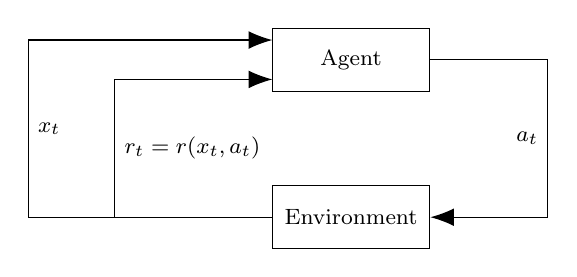
\begin{tikzpicture}

% definitions
\tikzstyle{box} = [rectangle, minimum width=2cm, minimum height=0.8cm, text centered, draw=black, fill=gray!0]

% the graph
\node (agent) [box] at (0,0) {\footnotesize Agent};
\node (env) [box, below of=agent, yshift=-1cm] {\footnotesize Environment};

\draw [-{Latex[length=3mm]}] 
    (env) -- +(-3,0) |- node[right, pos=0.25] {\footnotesize $r_t=r(x_t, a_t)$} ($(agent)+(-1, -0.25)$);

\draw [-{Latex[length=3mm]}] 
    ($(env)+(-1.1, 0)$) -- +(-3, 0) |- node[right, pos=0.25] {\footnotesize $x_t$} ($(agent)+(-1, 0.25)$);
    
\draw [-{Latex[length=3mm]}] 
    (agent) -- +(2.5,0) |- node[left, pos=0.25] {\footnotesize $a_t$} (env);

\end{tikzpicture}
\caption{Graphic representation of the reinforcement learning interaction. Every time the agent performs an action $a_t$, the environment modifies its state $x_{t-1}$ to $x_t$, computes the reward $r_t$ and sends both values to the agent, who uses them to optimize its policy.}
\label{fig:preliminaries:rl}
\end{center}
\end{figure}

\subsection{Neural Architecture Search}\label{sec:preliminaries:nas}

Neural Architecture Search (NAS) is the process of automating the design of neural networks. In order to formalize this definition, it is convenient to refer to the survey of~\citet{NASsurvey}, which characterize a NAS work with three variables: the \textit{search space}, the \textit{search strategy}, and the \textit{performance estimation strategy}. Figure~\ref{fig:preliminaries:nas} illustrates the interaction between these variables.

\begin{figure}[ht]
\begin{center}
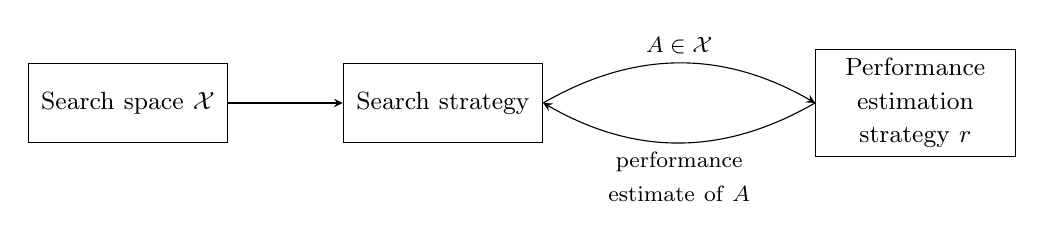
\begin{tikzpicture}

% definitions
\tikzstyle{box} = [rectangle, minimum width=2cm, minimum height=1cm, text width=2.3cm, text centered, draw=black, fill=gray!0]


\tikzstyle{arrow} = [->,>=stealth]


% the graph
\node (ss) [box] at (0,0) {\small Search space $\mathcal{X}$};
\node (st) [box, right of=ss, xshift=3cm] {\small Search strategy};
\node (pss) [box, right of=st, xshift=5cm] {\small Performance estimation strategy $r$};


\draw [arrow] (ss) -- (st);

\draw [arrow] (st.east) to [out=30,in=150] node [above,midway,text centered] {\footnotesize $ A \in \mathcal{X}$ } (pss.west);

\draw [arrow] (pss.west) to [out=210,in=330] node [below,midway, text width=2cm, text centered] {\footnotesize performance estimate of $A$} (st.east);



\end{tikzpicture}
\caption{An illustration of the three NAS variables interacting~\citep{NASsurvey}. At any moment during the search, the \textit{search strategy} samples an architecture $A$ from the \textit{search space} and sends it to the \textit{performance estimation strategy}, which returns the performance estimate. By design, the \textit{search space} and the \textit{performance estimation strategy} are named after the variables in Definition~\ref{def:preliminaries:rl} since they are typically equivalent in NAS within the reinforcement learning setting.}
\label{fig:preliminaries:nas}
\end{center}
\end{figure}

The \textit{search space} is the set of architectures considered in the search process. It is possible to define different spaces by constraining attributes of the networks, such as the maximum depth allowed, the type of layers to use, or the connections permitted between layers. A common abstraction inspired in popular networks is to separate the search spaces in \textit{chain} structures and \textit{multi-branch} structures that can be either \textit{complete} neural networks or \textit{cells} that can be used to build more complex networks, as illustrated in Figure~\ref{fig:preliminaries:ss}.

\begin{figure}[ht]
\begin{center}
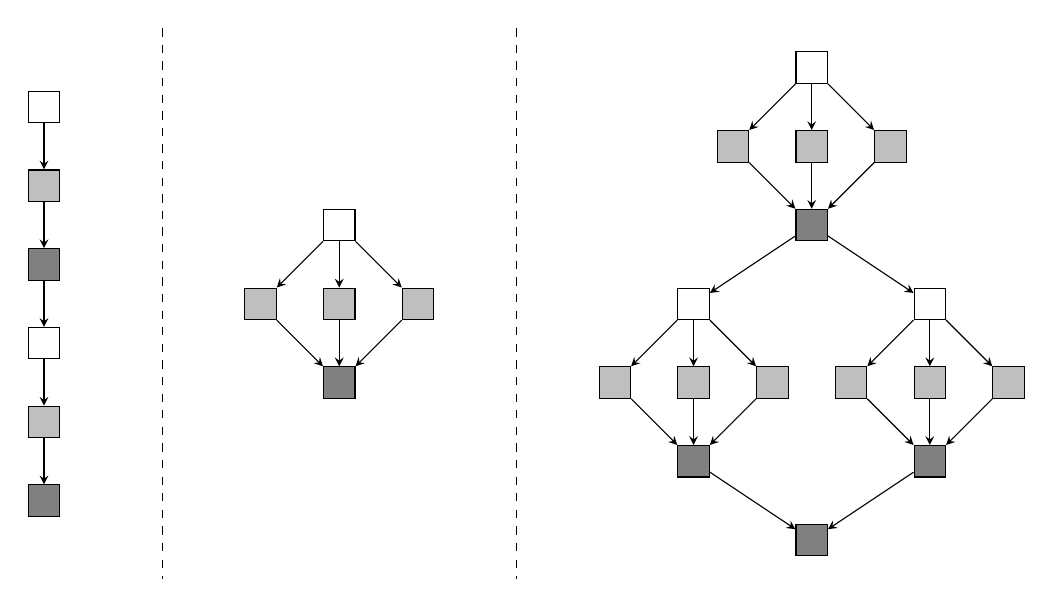
\begin{tikzpicture}

% definitions
\tikzstyle{squareA} = [rectangle, minimum width=0.4cm, minimum height=0.4cm, draw=black, fill=gray!0]

\tikzstyle{squareB} = [rectangle, minimum width=0.4cm, minimum height=0.4cm, draw=black, fill=gray!50]

\tikzstyle{squareC} = [rectangle, minimum width=0.4cm, minimum height=0.4cm, draw=black, fill=gray!100]

\tikzstyle{arrow} = [->,>=stealth]


% chain
\node (aa) [squareA] at (-0.75,-0.5) {};
\node (ab) [squareB, below of=aa] {};
\node (ac) [squareC, below of=ab] {};
\node (ad) [squareA, below of=ac] {};
\node (ae) [squareB, below of=ad] {};
\node (af) [squareC, below of=ae] {};


\draw [arrow] (aa) -- (ab);
\draw [arrow] (ab) -- (ac);
\draw [arrow] (ac) -- (ad);
\draw [arrow] (ad) -- (ae);
\draw [arrow] (ae) -- (af);

\draw[dashed] (0.75, 0.5) -- (0.75, -6.5);


% multi-branch cell
\node (ba) [squareA] at (3,-2) {};
\node (bb) [squareB, below of=ba, left of=ba] {};
\node (bc) [squareB, below of=ba] {};
\node (bd) [squareB, below of=ba, right of=ba] {};
\node (be) [squareC, below of=bc] {};

\draw [arrow] (ba) -- (bb);
\draw [arrow] (ba) -- (bc);
\draw [arrow] (ba) -- (bd);
\draw [arrow] (bb) -- (be);
\draw [arrow] (bc) -- (be);
\draw [arrow] (bd) -- (be);

\draw[dashed] (5.25, 0.5) -- (5.25, -6.5);


% multi-branch stack
\node (ca) [squareA] at (9,0) {};
\node (cb) [squareB, below of=ca, left of=ca] {};
\node (cc) [squareB, below of=ca] {};
\node (cd) [squareB, below of=ca, right of=ca] {};
\node (ce) [squareC, below of=cc] {};

\draw [arrow] (ca) -- (cb);
\draw [arrow] (ca) -- (cc);
\draw [arrow] (ca) -- (cd);
\draw [arrow] (cb) -- (ce);
\draw [arrow] (cc) -- (ce);
\draw [arrow] (cd) -- (ce);

\node (da) [squareA] at (7.5,-3) {};
\node (db) [squareB, below of=da, left of=da] {};
\node (dc) [squareB, below of=da] {};
\node (dd) [squareB, below of=da, right of=da] {};
\node (de) [squareC, below of=dc] {};

\draw [arrow] (da) -- (db);
\draw [arrow] (da) -- (dc);
\draw [arrow] (da) -- (dd);
\draw [arrow] (db) -- (de);
\draw [arrow] (dc) -- (de);
\draw [arrow] (dd) -- (de);

\node (ea) [squareA] at (10.5,-3) {};
\node (eb) [squareB, below of=ea, left of=ea] {};
\node (ec) [squareB, below of=ea] {};
\node (ed) [squareB, below of=ea, right of=ea] {};
\node (ee) [squareC, below of=ec] {};

\draw [arrow] (ea) -- (eb);
\draw [arrow] (ea) -- (ec);
\draw [arrow] (ea) -- (ed);
\draw [arrow] (eb) -- (ee);
\draw [arrow] (ec) -- (ee);
\draw [arrow] (ed) -- (ee);


\draw [arrow] (ce) -- (da);
\draw [arrow] (ce) -- (ea);

\node (f) [squareC, below of=de, right of=de, xshift=0.5cm] {};

\draw [arrow] (de) -- (f);
\draw [arrow] (ee) -- (f);


\end{tikzpicture}
\caption{Examples of networks belonging to different search spaces. On the left, a \textit{chain-structured} network. On the center, a \textit{multi-branch} network. On the right, the same multi-branch structure used as a \textit{cell} repeated multiple times to build a more complex network.}
\label{fig:preliminaries:ss}
\end{center}
\end{figure}


On the other hand, the \textit{search strategy} is simply the algorithm used to perform the search. The choices range from naive approaches such as random search to more sophisticated ones like reinforcement learning~\citep{BakerNAS, ZophNAS1}, evolutionary algorithms~\citep{AmoebaNet}, or gradient descent search~\citep{DARTS}.

Lastly, the \textit{performance estimation strategy} is the function used to measure the goodness of the sampled architectures. Formally, it is a function $R_{D}: \mathcal{X} \mapsto \mathbb{R}$ evaluating an architecture on a dataset $D$. The \textit{vanilla} estimation strategy is the test accuracy after training of a network, but different alternatives are proposed to try delivering an accurate estimate in a short time since expensive training creates a bottleneck in the search process.
\section{Related work}\label{sec:related}

Neural Architecture Search (NAS) is a broad field that can be approached from different perspectives, however we only study the area using reinforcement learning for the search of Convolutional Neural Networks (CNNs). For a cleaner presentation, in section~\ref{sec:related:summary} we sum up the relevant projects to our research, highlighting seven aspects per work: the search space explored, the performance estimation strategy, the policy optimization algorithm applied, the input datasets, the computational resources per experiment, whether or not the transferability of the discovered architecture was tested, and the main claims with respect to the numeric performance of the results. Next, in section~\ref{sec:related:analysis} we discuss the main contributions of those works and their differences, pointing to the features that inspire our research.

\subsection{Summary}\label{sec:related:summary}

We consider seven main investigations, which have contributed differently to the field of NAS via reinforcement learning\footnote{Some of these works address the generation of both Convolutional Neural Networks (CNNs) and Recurrent Neural Networks (RNNs). However, we omit the details for RNNs since they are out of the scope of this investigation.}. For their presentation we sort them in chronological order, and feature them by the seven attributes listed above.

\textbf{MetaQNN}~\citep{BakerNAS}. \emph{Search space}: chain-structured neural networks composed of convolutions, pooling operations and fully-connected layers. \emph{Performance estimation strategy}: test accuracy after 20 epochs of training. \emph{Policy optimization}: \textsc{Q-learning} with $\epsilon$-greedy exploration and memory replay. \emph{Input datasets}: Street View House Numbers (SVHN), CIFAR-10 and MNIST. \emph{Resources}: 10 GPUs running for 8-10 days per dataset. \emph{Transferability}: test the architecture generated for CIFAR-10 on the remaining two datasets with successful results. \emph{Performance}: This technique yielded to architectures that outperform other chain-structured networks and remain competitive against more complex architectures when considering the test error rate.


\textbf{NAS}~\citep{ZophNAS1}. \emph{Search space}: multi-branch CNNs that contain convolutions, rectified linear units and batch normalization. \emph{Performance estimation strategy}: test accuracy after 50 epochs. \emph{Policy optimization}: \textsc{Reinforce}, with a policy modeled as a Recurrent Neural Network (RNN). \emph{Input datasets}: CIFAR-10. \emph{Resources}: 800 GPUs running for 28 days. \emph{Transferability}: No studied. \emph{Performance}: The obtained architecture proved competitive against state-of-the-art models with respect to the test accuracy, and outperform them in terms of the test error rate and training speed.


\textbf{NASNet}~\citep{ZophNAS2}. \emph{Search space}: stacked multi-branch convolutional \textit{cells} containing convolutions, additions, concatenations, pooling and identities. \emph{Performance estimation strategy}: test accuracy after 50 epochs. \emph{Policy optimization}: \textsc{Reinforce}, with a policy modeled as a RNN. \emph{Input datasets}: CIFAR-10. \emph{Resources}: 500GPUs running for 4 days. \emph{Transferability}: the discovered cell is tested on the ImageNet dataset. \emph{Performance}: the results outperform state-of-the-art architectures for both accuracy and test error rate for CIFAR-10, and remain competitive for ImageNet with minor tuning.



\textbf{BlockQNN-V1}~\citep{BlockQNN}. \emph{Search space}: stacked multi-branch convolutional \textit{cells} composed of convolutions, additions, concatenations, pooling and identities. \emph{Performance estimation strategy}: test accuracy after 12 epochs only, with a penalization of the network's density and the number of Floating Point Operations (FLOPs). \emph{Policy optimization}: \textsc{Q-learning} with $\epsilon$-greedy exploration. \emph{Input datasets}: CIFAR-10. \emph{Resources}: 32 GPUs running for 3 days. \emph{Transferability}: the discovered cell is tested on ImageNet. \emph{Performance}: competitive results on CIFAR-10 regarding the test error rate and \textit{very} competitive on ImageNet with minor tuning.
 
\textbf{BlockQNN-V2}~\citep{BlockQNN}. \emph{Search space}: stacked multi-branch convolutional \textit{cells} composed of convolutions, additions, concatenations, pooling and identities. \emph{Performance estimation strategy}: pre-trained neural network that estimates the accuracy of any network based on its complexity. \emph{Policy optimization}: \textsc{Q-learning} with $\epsilon$-greedy exploration. \emph{Input datasets}: CIFAR-10. \emph{Resources}: 1 GPU running for 20 hours \emph{Transferability}: the discovered cell is tested on ImageNet. \emph{Performance}: lower but yet competitive results with respect to BlockQNN-V1.

\textbf{Path-level Network Transformation}~\citep{PathNAS}. \emph{Search space}: morphisms of a pre-defined network via Net2Net-like transformations on convolutions and pooling layers. \emph{Performance estimation strategy}: test accuracy after 20 epochs with re-usage of weights of the network before transformation. \emph{Policy optimization}: \textsc{Reinforce} with policy represented by a tree-structured LSTM. \emph{Input datasets}: CIFAR-10. \emph{Resources}: 200 GPU hours. \emph{Transferability}: the discovered network is tested on ImageNet. \emph{Performance}: excel state-of-the-art human-designed and NAS-designed networks on both datasets.

\textbf{ENAS}~\citep{ENAS}. \emph{Search space}: all sub-graphs from a fully-connected Directed Acyclic Graph (DAG) of 7 nodes, where each node can be a convolution, depth-wise separable convolution, max pooling, and average pooling. \emph{Performance estimation strategy}: test accuracy after 150 epochs of training. \emph{Policy optimization}: \textsc{Reinforce} with a policy represented by a RNN. \emph{Input datasets}: CIFAR-10. \emph{Resources}: 1 GPU running for 7 hours. \emph{Transferability}: not studied. \emph{Performance}: the discovered network performed almost as good as the NASNet~\citep{ZophNAS2} in terms of the test error (0.24\% difference only).


\subsection{Analysis}\label{sec:related:analysis}

The works above display the complexity of Neural Architecture Search (NAS), in the sense that  This is, while one would hope to solve the problem as a whole, there is a number of factors that impede to satisfy this ambition, forcing researchers to settle for particular objectives.

Perhaps the biggest of those factors is the cost of training neural networks. In a typical reinforcement learning setting, thousands of steps are performed to allow the agent to learn a policy based on rewards from its interaction with the environment at each step. For NAS, this reward is, in principle, the accuracy after training on a test set for each of the sampled networks, meaning that thousands of train-evaluation procedures are performed per experiment. An example of the expensiveness of this approach is the long training reported by~\citet{ZophNAS1}, where the computational cost is beyond the possibilities of many researches: hundreds of GPUs running during almost a month. In an attempt to avoid the bottleneck caused by this costly procedure, different relaxations are proposed to estimate the performance of the networks, rather than performing expensive training procedures: reduce the number of epochs~\citep{BakerNAS,BlockQNNprev}, constrain the search space to generate similar networks that can re-use weights and allow for a shorter training~\citep{PathNAS}, or skip the training of the networks by predicting their performance~\citep{BlockQNN}. Perhaps appealing at first, these relaxations might cause an incorrect assessment of the real performance of the architectures, favouring the ones that might not be as good as the estimation suggests. This observation was considered in the BlockQNN project~\citep{BlockQNN}, where the reward function takes the accuracy after training with early-stop but penalizes it with the network's density and FLOPs, making the reward more relevant to the final performance of the architectures.

A second factor influencing the performance of the NAS strategies is the definition of the search space. In that regard, some researchers opt for a clearly diverse space~\citep{ZophNAS1,ZophNAS2,BlockQNN} and others for a more compact one~\citep{PathNAS,ENAS}. We make the observation that the relaxations on the search space seem highly related to the computational resources required, where a less restricted space usually requires more computational power. Concrete examples of this observation are the NAS~\citep{ZophNAS1} and NASNet~\citep{ZophNAS2} projects, where the drastic difference in the computational cost is claimed to be caused by the reduction of the search space in NASNet, since the same reinforcement learning setting is applied for both of the experiments. Another work that supports our observation is MetaQNN~\citep{BakerNAS}, where the search space is restricted to chain-structured networks avoiding the complexity of a multi-branch space and resulting in a more feasible experiment with respect to the number of GPUs and days required per experiment, even though the cost of the training-evaluation procedure per network is still considerable. Lastly, ENAS~\citep{ENAS} shows that a more drastic reduction of the search space leads to an impressively shorter duration of the experiments with only 1 GPU. ENAS designs a search space modeled as a super graph where the sampled architectures are sub-graphs only. In fact, the design of this search space has been shown to be the primary cause of the performance of the method and not the the reinforcement learning procedure~\citep{ENASbad}, meaning that the space itself contains well-performing networks that could be explored with search strategies other than reinforcement learning and yet leading to similar performance.

From the analysis above we make two notes. Firstly, it can be seen that there exists a trade-off between the search space and the performance estimation strategy used in the experiments. This is, when defining a more compact search space there is more chance to use the actual accuracy after a considerable number of training epochs, whereas when considering a more complex one few epochs are preferred to avoid the bottleneck of the train-evaluation procedures. Secondly, the definition of the search space constrains the ultimate goal of the policy that is to be learned, i.e. a less restricted space usually targets for a policy that is optimized to deal with all aspects of the design of the architectures, and a reduced one serves only as a simple search method that can potentially be replaced, loosing the conceptual benefits of reinforcement learning. %Based on this, we consider that among all the studied works BlockQNN-V1~\citep{BlockQNN} provides the best framework for NAS via reinforcement learning, since it provides a complex search space and a performance estimation strategy that takes in consideration the real performance of the network and reduces the bias of the reward.

%Other recent approaches that have been applied to NAS are those of~\citet{DARTS} and \cite{ProgressiveNAS}.
\section{Methodology}\label{sec:methodology}

The methodology that we set for this work can be split in two: the Neural Architecture Search (NAS) artifacts and the reinforcement learning framework. 
%In this section we elaborate on each of these elements and we present the setting of our experiments.
In a nutshell, we make use of the deep-meta reinforcement learning framework proposed by~\citet{LtRL} and~\citet{RL2} to learn from a distribution of Markov Decision Processes\footnote{In this report, we use the terms MDPs and environments as equivalents.} (MDPs), rather than from a single MDP as it is done in a standard reinforcement learning setting. The MDPs that we consider are instances of the meta-dataset collection assembled by~\citet{MetaDataset}, which we use for standard classification tasks. With respect to the NAS elements, we designed a search space similar to the one in BlockQNN~\citep{BlockQNN} and we apply the same performance strategy they proposed. Under this setting we set two main experiments: a) generate both chain-structured and multi-branch networks, for which we test their transferability on a new dataset, and b) test the transferability of the learned policy to solve a new MDP (i.e. an image classification task on a new dataset). We compare our results with those generated using standard Q-learning with the same search space and performance estimation strategies, but using CIFAR-10 as the only MDP.

In the remaining of this section we deepen into these components and present the setting for our experiments.

\subsection{The Neural Architecture Search elements}\label{sec:methodology:nas}

As it was sketched out by~\cite{NASsurvey}, Neural Architecture Search (NAS) can be studied from three different flanks: the search strategy, the search space, and the performance estimation strategy. In this section we elaborate on the latter two, which follow the base methodology of BlockQNN~\citep{BlockQNN} with some minor modifications.

\subsubsection{The search space}\label{sec:methodology:ss}

Our search space is highly inspired by the BlockQNN project~\citep{BlockQNN}, which defines it as all possible architectures that can be generated by sequentially stacking elements from a so-called Network Structure Code (NSC) space that is described in Table~\ref{tab:nas:nsc}. Originally, the NSC space contains 7 elements, each with a pre-defined range for an associated hyperparameter and the allowed incoming connections (i.e. the inputs), nevertheless we ignore the \textit{identity} operation, since we consider it redundant under our setting.

In principle, this search space does not impose any constraint upon the allowed connections in the architecture as long as they are valid, making it possible to explore both multi-branch and chained structures; however, to make the search more efficient we introduce minor restrictions depending on the type of structure that is considered. In the case of the chained-structured networks we ignore the \textit{concatenation} and \textit{addition} operations, since only one predecessor is considered to build the chain. On the other hand, to avoid high-dimensional blocks that can cause memory issues for the multi-branch structures, we do not consider the \textit{concatenation} operation as a possible action during the design of the networks, but instead we use it as a merge operation when the resulting network has more than one leaf.


% Please add the following required packages to your document preamble:
% \usepackage{booktabs}
\begin{table}[ht]
\centering
\begin{tabular}{@{}ccccc@{}}
\toprule
\textbf{Name}   & \textbf{Type} & \textbf{Kernel size} & \textbf{Predecessor 1} & \textbf{Predecessor 2} \\ \midrule
Convolution     & 1             & \{1, 3, 5\}          & \textbf{K}             & $\emptyset$            \\
Max Pooling     & 2             & \{1, 3\}             & \textbf{K}             & $\emptyset$            \\
Average Pooling & 3             & \{1, 3\}             & \textbf{K}             & $\emptyset$            \\
Addition        & 5             & $\emptyset$          & \textbf{K}             & \textbf{K}             \\
Concatenation   & 6             & $\emptyset$          & \textbf{K}             & \textbf{K}             \\
Terminal        & 7             & $\emptyset$          & $\emptyset$            & $\emptyset$            \\ \bottomrule
\end{tabular}
\caption{The search space presented in Neural Structure Code (NSC) format, as in the original BlockQNN paper~\citep{BlockQNN}. On purpose, the \textbf{Type} 4 code is missing since we preserved the original enumeration. The values in the set \textbf{K} are dependent on the level of the network, i.e. $\textbf{K} = \{1, 2, \dots , \text{current layer index} - 1 \}$ }
\label{tab:nas:nsc}
\end{table}

We note that this space is flexible to search for complete architectures or \textit{cells} only. For our experiments, we take advantage of this as it is presented in section~\ref{sec:methodology:experiments}.

\subsubsection{The performance estimation strategy}\label{sec:methodology:pss}

We use a penalized early-stop accuracy as the one in BlockQNN~\citep{BlockQNN}, as described in equation~\ref{eq:pes}, where $\mu, \rho \in [0, 1]$ are weights for the penalization terms, FLOPs is the number of floating point operations of the block, and Density is the edge number divided by the dot number when treating the network as a Directed Acyclic Graph (DAG). 

We prefer this strategy over others found in literature because of our interest in training the network with few epochs to save computing time during the learning process. Furthermore, this penalized version has been shown useful to compensate the pitfall of early-stop that may underestimate good architectures. For a deeper study, we refer to the original paper.

\begin{equation}\label{eq:pes}
reward = \text{ACC}_\text{EarlyStop} - \mu \log(\text{FLOPs}) - \rho \log(\text{Density})
\end{equation}

\subsection{The reinforcement learning framework}\label{sec:methodology:rl}

%by interacting with the environment a so-called \textit{agent} learns the distribution of state-actions pairs over the \textit{reward} domain, allowing to accomplish a goal on the environment in a guided way. In other words, the agent is able to capture the convenience of the actions at specific states, so that it can efficiently achieve its goal.

It has already been stressed that our research uses reinforcement learning as the search strategy to address the NAS problem. 
%The choice is not arbitrary, and we base it on the theoretical advantages of reinforcement learning over other goal-directed learning approaches~\citep{RLIntroBook}. 
Particularly, we are interested in exploiting the framework's foundation: the distribution of \textit{state}-\textit{action} pairs over the \textit{reward} domain that is learned from the interaction of the \textit{agent} with the \textit{environment}. We aim to strengthen that distribution by making use of a deep-meta-reinforcement learning framework~\citep{LtRL, RL2}, which is different from the standard reinforcement learning in two main aspects: 1) the agent is challenged to face more than one environment, and 2) the distribution is now dependant on the whole history of state, actions and rewards; instead of the simple state-action pairs. The distribution is learned with the help of a \textit{policy} modeled with a Recurrent Neural Network (RNN) that thanks to its internal dynamics and the learning setting, is able to adapt to different environments and achieve its goal efficiently.

When applied to NAS this extension has two main implications. The first one is that by letting the agent learn from different environments (i.e. datasets), the resulting architecture after training is built based on a more complex distribution that takes into account the current environment and the ``long-term" effect of every executed action (change in the architecture), leading to a better design of the architecture. The second implication is that the resulting policy can be trained on a previously unseen environment (i.e. a new dataset) to design an \textit{ad hoc} architecture in a faster way, since the policy already has a ``general" distribution embedded in the RNN, and therefore the new training will only integrate the information specific to the new environment.

Here below, we formally present the version of deep-meta reinforcement learning that we implement, which is primarily based on the methodology of~\citet{LtRL}, with a small modification taken from the parallel and complementary research of~\citet{RL2}.

\subsubsection{Formalization}\label{sec:methodology:rl:formal}

Let $\mathcal{D}$ be a distribution over a set of Markov Decision Processes (MDPs). An appropriately structured agent, embedding a recurrent neural network, is trained by interacting with a sequence of MDP environments (also called \textit{tasks} or \textit{trials}) through episodes. At the start of a new task $m \sim \mathcal{D}$ an initial state for this task is sampled, and the internal state of the agent (i.e., the pattern of activation over its recurrent units) is reset. The agent then starts a number $n$ of episodes for which it executes its action-selection strategy for a certain number of discrete time-steps. At each step $t$ an action $a_t \in A$ is executed as a function of the whole history $H_t = \{x_0, a_0, r_0, . . . , x_{t-1}, a_{t-1}, r_{t-1}, x_t\}$ of the agent interacting in the MDP $m$ during the current episode (set of states $\{x_s\}_{0 \leq s \leq t}$, actions $\{a_s\}_{0 \leq s < t}$, and rewards $\{r_s\}_{0 \leq s < t}$ observed since the beginning of the first episode, when the recurrent unit was reset). The network weights are trained to maximize the sum of observed rewards over all steps and episodes.

After training, the agent's policy is fixed (i.e. the weights are frozen, but the activations are changing due to input from the environment and the hidden state of the recurrent layer), and it is evaluated on a set of MDPs that are drawn either from the same distribution $\mathcal{D}$ or slight modifications of that distribution (to test the generalization capacity of the agent). The internal state is reset at the beginning of the evaluation of any new task.

% \subsubsection{Specifics}

\subsubsection{The action space}\label{sec:methodology:rl:as}

Contrarily to the works studied in section~\ref{sec:related}, we formulate the action space as a discrete space similar to those of the Atari environments. Table~\ref{tab:rl:as} shows this space in detail. 

In particular, given the maximum number $E$ of elements in the network, we model the space as an matrix of shape $E \times 5$, where the 5 is length of the NSC presented in section~\ref{sec:methodology:ss}. In this representation, we allow the agent to control a pointer that can be shifted upwards or downwards to select the predecessor. As a consequence, the agent is able to learn the best way to move this pointer to increase its accumulated reward during the trial.


% Please add the following required packages to your document preamble:
% \usepackage{booktabs}
\begin{table}[ht]
\centering
\begin{tabular}{@{}ccc@{}}
\toprule
\textbf{Structure type}                                         & \textbf{Encoding}                            & \textbf{Description}                                                                                                                            \\ \midrule
\begin{tabular}[c]{@{}c@{}}Chained,\\ Multi-branch\end{tabular} & convolution\_k-\{1, 3, 5\}\_pred1-L\_pred2-0 & \begin{tabular}[c]{@{}c@{}}Convolution with a kernel in\\ set \{1, 3, 5\}. Predecessor1 is\\ always the last layer (L).\end{tabular}            \\
\begin{tabular}[c]{@{}c@{}}Chained,\\ Multi-branch\end{tabular} & maxpooling\_k-\{1, 3\}\_pred1-L\_pred2-0     & \begin{tabular}[c]{@{}c@{}}Max-pooling with a pool size\\ in set \{1, 3\}. Predecessor1 is\\ always the last layer (L).\end{tabular}            \\
\begin{tabular}[c]{@{}c@{}}Chained,\\ Multi-branch\end{tabular} & avgpooling\_k-\{1, 3\}\_pred1-L\_pred2-0     & \begin{tabular}[c]{@{}c@{}}Average-pooling with a pool\\ size in set \{1, 3\}. Predecessor1\\ is always the last layer (L).\end{tabular}        \\
\begin{tabular}[c]{@{}c@{}}Chained,\\ Multi-branch\end{tabular} & terminal\_k-0\_pred1-0\_pred2-0              & The terminal state.                                                                                                                             \\
Multi-branch                                                    & add\_k-0\_pred1-L\_pred2-BL                  & \begin{tabular}[c]{@{}c@{}}Addition with Predecessor1\\ and Predecessor2 controlled\\ by an internal pointer in the\\ environment.\end{tabular} \\
Multi-branch                                                    & predshift\_p-\{1, 2\}\_op-\{U, D\}           & \begin{tabular}[c]{@{}c@{}}Move the predecessors (1 or 2)\\ upwards (U) or downwards (D).\end{tabular}                                          \\ \bottomrule
\end{tabular}
\caption{caption}
\label{tab:rl:as}
\end{table}

\subsubsection{The environments}\label{sec:methodology:rl:datasets}

In section~\ref{sec:methodology:rl:formal} there is an assumption of working with a distribution $\mathcal{D}$ of MDPs from which different environments are sampled. In our case, this distribution is composed of of image datasets from the meta-dataset collection~\citep{MetaDataset} that is originally composed of 10 datasets that we reduce to 9. Originally, the meta-dataset is intended to improve the performance of \textit{meta} models for few-shot classification and therefore, we perform some modifications for our tasks that are standard classification tasks.

In specific, we define a different train-validation usage of the datasets and we set an order in the usage of the environments for the different trials needed for deep meta-reinforcement learning. The order imposed is based on the complexity of the classification tasks, where we consider simpler tasks the ones with few classes and relatively few observations, so that the agent can gradually learn to behave on different environments. We consider this order important to facilitate the learning curve of the agent, since intuitively complex datasets could lead to low rewards related to the complexity of the task more than to the effectiveness of the actions performed. Table~\ref{tab:meta-dataset} shows our usage of the meta-dataset.

We consider important to note that in their plain versions, these datasets have different shapes (width and height). To solve this, we stick to the original meta-dataset pre-processing that resizes the images to a shape of $84 \times 84$ with the 3 RGB channels using a bilinear interpolation, so that all images in the super collection share the same dimensions.

\begin{table}[ht]
\centering
\begin{tabular}{@{}cccccc@{}}
\toprule
Dataset ID    & Dataset name                              & Usage      & Trial        & N classes & N observations \\ \midrule
aircraft      & FGVC-Aircraft                             & Train      & 3            & 100       & 10000          \\
cu\_birds     & CUB-200-2011                              & Train      & 5            & 200       & 11788          \\
dtd           & Describable Textures                      & Train      & 2            & 47        & 5640           \\
fungi         & FGVCx Fungi                               & Train      & 7            & 1394      & 89760          \\
omniglot      & Omniglot                                  & Validation & -            & 1623      & 32460          \\
quickdraw     & Quick, Draw!                              & Train      & 6            & 345       & 50426266       \\
traffic\_sign & German Traffic Sign                       & Train      & 1            & 43        & 39209          \\
vgg\_flower   & VGG Flower                                & Train      & 4            & 102       & 8189           \\
ilsvrc\_2012  & ImageNet                                  & Validation & -            &           &                \\ \bottomrule
\end{tabular}
\caption{Subset of the meta-dataset~\citep{MetaDataset} that we use for the experiments. Three main things can be noted: a) the MSCOCO dataset was removed, b) the datasets for train and validation were modified with respect to the original work, and c) an order in the trials was established to allow the agent to gradually face more complex datasets.}
\label{tab:meta-dataset}
\end{table}

% TODO: explain the 

\subsection{Software specifics}\label{sec:methodology:software}

In an effort to make our research open, we put the source code developed for this project publicly available at https://github.com/gomerudo/nas-dmrl. This development uses TensorFlow~\citep{tensorflow} as the framework for the building and training of the architectures, the OpenAI baselines~\citep{openaibaselines} for the reinforcement learning algorithm, and includes an OpenAI Gym~\citep{openaigym} environment that we developed and named \textsc{nasgym}, which can be used with any of the available OpenAI baselines' algorithms. We believe that this is an important contribution that will allow to study our framework with variations that are programmatically easy to implement, and it will inspire future research for NAS.

\subsection{Experiments}\label{sec:methodology:experiments}

\subsubsection{The baseline}\label{sec:methodology:experiments:baseline}

\textbf{TODO: Still we will need to define the parameters used for Q-learning.}

\section{Evaluation framework}\label{sec:software}

The current Neural Architecture Search (NAS) solutions lack a crucial element: an open-source framework for reproducibility and further research. Specifically for NAS with reinforcement learning, it would be desirable to build on a programming interface that allows researchers to explore the effect of different algorithms on the same NAS environment. In an attempt to fill this gap, we have developed the \textsc{nasgym}\footnote{Source code available at: github.com/gomerudo/nas-env}, a python OpenAI Gym~\citep{openaigym} environment that can jointly be used with all the reinforcement learning algorithms exposed in the OpenAI baselines~\citep{openaibaselines}. 

We make use of the object-oriented paradigm to abstract the most essential elements of NAS as a reinforcement learning problem, resulting in a system that can be extended to perform new experiments, as displayed in Figure~\ref{fig:software:architecture}. Although the defaults in the \textsc{nasgym} are the elements in our methodology, the system allows us to easily modify the key components, such as the performance estimation strategy, the action space, or the Neural Structure Code space. We also provide an interface to use a database of experiments that can help to store previously computed rewards, thus reducing the computation time of future trials. All the deep learning components are built with TensorFlow v1.12~\citep{tensorflow}.



\begin{figure}[ht]
\begin{center}
\begin{tikzpicture}

% definitions
\tikzstyle{boxA} = [rectangle, dashed, minimum width=2cm, minimum height=1cm, text centered, draw=black, fill=gray!0]
\tikzstyle{boxempty} = [rectangle, minimum height=1cm, text width=3cm, text centered, fill=gray!0]



\tikzstyle{arrow} = [->,>=stealth]


% box top
\draw (-4, 0) -- (-4, -4); % left
\draw (-4, 0) -- (-3, 0); % topA
\node at (-2.2, 0){\textsc{nasgym}}; % Label
\draw (-1.35, 0) -- (5, 0); % topB
\draw (-4, -4) -- (5, -4); % bottom
\draw (5, 0) -- (5, -4); % right


\node (nasenv) [boxA] at (0.75, -1) {\small \textsc{DefaultNasEnvironment}};

\node (datahandler) [boxA, below of=nasenv, yshift=-1cm, xshift=-2cm] {\small \textsc{DatasetHandler}};

\node (dbexperiments) [boxA, below of=nasenv, yshift=-1cm, xshift=2cm] {\small \textsc{DbInterface}};





\node (nscdef) [boxempty, left of=nasenv, xshift=-6cm] {\faFileCodeO \\ \small NSC \\definition file};

\node (config) [boxempty, below of=nscdef, yshift=-1cm] {\faFileCodeO \\ \small Hyper-parameters values};

\node (tfrecords) [boxempty, below of=datahandler, yshift=-1cm] {\faFilesO \\ \small TFRecords files};

\node (db) [boxempty, below of=dbexperiments, yshift=-1.2cm] {\faDatabase \\ \small Database of \\ experiments};


\draw [arrow] (nscdef) -- (nasenv);
\draw [arrow] (config) -- (nasenv.west);
\draw [arrow] (tfrecords) -- (datahandler);
\draw [arrow] (db) -- (dbexperiments);


\end{tikzpicture}
\caption{An sketch of the system built to perform our research. The \textsc{nasgym} package contains a default NAS environment whose states and actions are designed according to the Neural Structure Code (NCS) space defined in a \textit{.yml} file. The hyperparameters for all the machine learning components are defined in a \textit{.ini} file. Internally, the environment makes use of a dataset handler that reads TFRecords files and sends them as inputs to the neural architectures. A simple database of experiments is used to store experiments in a local file, although the logic can be easily be extended to support a more robust database system.}
\label{fig:software:architecture}
\end{center}
\end{figure}

Additionally to the \textsc{nasgym}, we implement the meta version of the A2C algorithm on top of the OpenAI baselines\footnote{Source code available at: github.com/gomerudo/openai-baselines}. We believe that this software engineering effort will help to compare, reproduce, and develop future research in NAS.

\section{Experiments}\label{sec:experiments}

% We empirically assess the quality of the networks designed by the agent through episodes, the ability of the agent to adapt to each environment, and the runtimes of the training trials.

To evaluate our framework, we conduct three experiments. The first two aim to study the behavior of the agent when challenged to design chain-structured networks, and the third one is intended to observe its behavior in the multi-branch setting. We empirically assess the quality of the networks designed by the agent through episodes, the ability of the agent to adapt to each environment, and the runtimes of the training trials.

\subsection{Chain-structured networks} \label{sec:experiments:chain}

% \subsubsection*{Experiment 1: the learning evolution during training}
\textbf{Experiment 1: evolution during training.} The agent learns from the three train environments listed in Table~\ref{tab:methodology:environments:datasets}, using deep meta-RL. It starts in the \textit{omniglot} environment, continues in \textit{vgg\_flower}, and finishes in \textit{dtd} so that it faces increasingly harder classification tasks (see Appendix~\ref{app:datasets}), and the policy learned in one environment is reused in the next one. The agent interacts with each environment for $t_{max}=8000$, $t_{max}=7000$, and $t_{max}=7000$, respectively so that the agent spends more time in the first environment to develop its initial knowledge.
%The main interest is in observing the evolution of the best rewards obtained through episodes. 
We compare against two baselines: random search and \textsc{DeepQN} with experience replay, where the agent learns a new policy on each environment (i.e., it does not re-use the policy between trials) for $t_{max}=6500, 5500, \text{ and }7000$, respectively. Due to resources and time constraints, all $t_{max}$ values were empirically selected according to the behaviour of the rewards (see Section~\ref{sec:results}). The most relevant hyper-paremeters are set as follows:

\begin{itemize}
    \setlength\itemsep{0em}
    \setlength\parskip{0pt}
    \item[-] \textsc{Environment}
        \begin{itemize}
            \setlength\itemsep{0em}
            \item[-]  $d=10$. The maximum depth of a neural architecture.
            \item[-] $\tau=10$. The maximum length of an episode.
        \end{itemize}
    \item[-] \textsc{A2C hyper-parameters}
    \begin{itemize}
        \setlength\itemsep{0em}
        \setlength\parskip{0pt}
        \item[-] $j=5$. The number of steps to perform before updating the A2C parameters (see Equation~\ref{eq:methodology:rl:poa:gradient}). We set the value to half the maximum depth of the networks to allow the agent to learn before the termination of an episode.
        \item[-] $\gamma=0.9$. The discount factor for the past actions.
        \item[-] $\eta=0.01$. The default in the OpenAI baselines~\citep{openaibaselines}.
        \item[-] $\alpha=0.001$. The A2C learning rate set as in \textit{Learning to reinforcement learn}~\citep{LtRL}.
    \end{itemize}
    \item[-] \textsc{DeepQN}
    \begin{itemize}
        \setlength\itemsep{0em}
        \setlength\parskip{0pt}
        \item[-] Experience $\text{buffer size}=\frac{t_{max}}{2}$. 
        \item[-] Target model's $\text{batch size} = 20$.
        \item[-] $\epsilon$ with linear decay from 1.0 to 0.1. The parameter controlling the exploration of the agent.
        \item[-] $\alpha=0.0005$. The default learning rate in the OpenAI baselines~\citep{openaibaselines}.
    \end{itemize}
    \item[-] \textsc{Training of the sampled networks}
    \begin{itemize}
        \setlength\itemsep{0em}
        \setlength\parskip{0pt}
        \item[-] $\text{batch size}=128$.
        \item[-] $\text{epochs}=12$. The value used in BlockQNN~\citep{BlockQNN}.
    \end{itemize}
\end{itemize}

% \textsc{DeepQN}: $\alpha=0.0005$, $\text{buffer size}=\frac{t_{max}}{2}$, target model's $\text{batch size} = 20$, and $\epsilon$ with linear decay from 1.0 to 0.1. \textsc{Environment}: $d=10$, $\tau=10$. \textsc{Training of the sampled networks}: $\text{batch size}=128$ and $\text{epochs}=12$.

\textbf{Experiment 2: evaluation of the policy.} We fix the policy obtained in Experiment 1. The agent interacts with the evaluation environments, \textit{aircraft} and \textit{cu\_birds}, and deploys its decision-making strategy to design a neural architecture for each dataset. The interaction runs for $t_{max}=2000$ to study the performance of the policy in short evaluation trials. At the end of the interaction, we select the best two architectures per environment (i.e., the ones with the highest reward) and train them on the same datasets but applying a more intensive procedure as follows. First, we augment the capacity of the architectures by changing the number of filters in the convolution layers according to the layer's depth; i.e., $\text{number of units}=2^{4+i}$ with $i$ being the current count of convolutions while building the network  (e.g., $\text{number of units}=32 \rightarrow 64 \rightarrow 128$). Second, we stack the prediction module as described in Section~\ref{sec:methodology:nas:pss}, but we increase the number of units in the first dense layer to 4096, we use a learning rate with exponential decay, and we train the network for 100 epochs. Since the datasets that we use are resized to a shape of 84x84x3, it is not fair to compare our resulting accuracy values with those of state-of-the-art architectures that assume a higher order of shape~\citep{FineGrained2, FineGrained3, FineGrainedResults}, and neither is to train our networks (which are designed for a given input size) with bigger images. Hence, based on the baselines of~\citet{FineGrainedResults}, we use a VGG-19 network~\citep{VGGPaper} with only two blocks as our baseline on both datasets.


\subsection{Multi-branch networks} \label{sec:experiments:multibranch}


\textbf{Experiment 3: training on a more complex environment.} In this experiment, we extend the search space to multi-branch architectures. We consider the \textit{omniglot} environment only. The goal here is to observe the ability of the agent to design multi-branch networks through time; i.e., the number of multi-branch structures generated through training. The interaction runs for $t_{max}=20000$ time-steps because more exploration is required due to the larger action space. The hyper-parameters are the same as in Experiment 1, except that $\tau=20$ and $j=10$ because the trajectories are longer due to the shifting of the pointers controlling the predecessors, and $\text{batch size}=64$ because the concatenation operation can generate networks that require more space in memory. We train the agent from scratch two times varying the parameter $\sigma \in [0.0, 0.1]$ (see Section~\ref{sec:methodology:rl:environments}) to study its effect encouraging the generation of multi-branch structures.

\section{Results}\label{sec:results}
\section{Conclusions and future work}\label{sec:conclusions}

% TODO: work in progress
In this work, we presented the first application of deep meta-RL in the NAS setting. Firstly, we investigated the advantages of deep meta-RL against standard RL on the relatively simple scenario of chain-structured architectures. Despite resource limitations (1 GPU only), we observed that a policy learned using deep meta-RL can be transferred to other environments and quickly designs architectures with higher and more consistent accuracy than standard RL. Nevertheless, standard RL outperforms meta-RL when both learn a policy from scratch. We also note that the meta-RL agent exhibited adaptive behavior during the training, changing its strategy according to the dataset in question.  Secondly, we analyzed the adaptability of the agent during evaluation (i.e., when the policy's weights are fixed) and the quality of the networks that it designs for previously unseen datasets. In our experiment, the agent was not able to adapt its strategy to different environments, but the performance of the networks delivered was better than the performance of a human-designed network, showing that the knowledge developed by our agent in the training environments is meaningful in others. Thirdly, we extended our approach to a more complex NAS scenario with a multi-branch search space. In this setting, the meta-RL agent was not able to deeply explore the multi-branch search space designed and settled for chain-structured networks instead.

We conclude that deep meta-RL does provide an advantage over standard RL when transferring is enabled, and it can adapt to environments during training. 
From all these observations, we advice future work to focus on pre-training the agent on more environments and for longer to perform better on unseen environments, hyper-parameter tuning of the deep meta-RL (specifically to control the exploration of the agent), exploring other RL algorithms (next to AC2) in a meta-RL framework, refining or redesigning the datasets used to avoid low accuracy values that might affect the learning of the agent, proposing other performance estimation strategies than help to reduce the cost of NAS, and redesigning the action space for the case of a multi-branch search space. 

We conclude that deep meta-RL does provide an advantage over standard RL when transferring is enabled, and it can adapt to different environments during training. Moreover, we believe that it is possible to strengthen the deep-meta RL framework in future work. Specifically, we propose to investigate the following aspects:



Additionally, we recommend to benchmark other RL algorithms on the same NAS environments. We believe that the system that we developed (see Section~\ref{sec:software}) will help to encourage research in these directions.

%and evaluation of the methodology in a more complex search space such as multi-branch networks.

% \textbf{TODO:} Add  conclusions. In short:
% \begin{itemize}
%     \item deep meta-RL shows efficient during training
%     \item The policy does not adapt during evaluation, but it designs good architectures, considering the hardness of the datasets.
%     \item Exploration is achieved
%     \item multi-branch structures are not explored, the framework should be modified. (Still thinking of possibilities: maybe re-formulate the rewards for the shifting operations, predict the layer from the policy - which is similar to NAS by Google.)
% \end{itemize}

% Future work:
% \begin{itemize}
%     \item More training
%     \item hyper-parameter tuning; specially the entropy regularizer
%     \item explore other RL algorithms
%     \item explore other datasets to avoid low accuracies that might trap the agent
%     \item explore alternatives for multi-branch structures
    
% \end{itemize}

% Acknowledgements should go at the end, before appendices and references

% \acks{We would like to acknowledge support for this project
% from the National Science Foundation (NSF grant IIS-9988642)
% and the Multidisciplinary Research Program of the Department
% of Defense (MURI N00014-00-1-0637). }

\acks{J. Gomez: to the \textit{Eindhoven University of Technology}, the \textit{Dutch Ministry of Education, Culture and Science} and the \textit{Consejo Nacional de Ciencia y Tecnologia} (CONACyT, Mexico) for the financial support during the completion of the master's program for which this project was conducted. To dr. ir. Joaquin Vanschoren, for his continuous support and guidance during the execution of the project. To the \textit{SURF} cooperative for kindly providing the required computational resources.} %To my family: L, J, and P.}

\vskip 0.2in
\bibliography{sample}

\newpage
\appendix
% \section{A concise survey of Neural Architecture Search with reinforcement learning}\label{app:related}

When addressing Neural Architecture Search (NAS) with reinforcement learning the main interest of the current research is usually that of obtaining an architecture that achieves state-of-the-art \textit{performance} on baseline datasets however, other aspects are also relevant in a NAS implementation. In this section we systematically survey the existing reinforcement learning works using seven variables that affect their utility: the \textit{search space}, the \textit{performance estimation strategy}, the \textit{reinforcement learning algorithm}, the \textit{input datasets}, the computational \textit{resources} demanded, the \textit{transferability properties} of the methodologies, and the \textit{performance} of the discovered architectures. For the sake of conciseness we omit other strategies for NAS, but we refer the reader to the survey of~\citet{NASsurvey} where approaches such as evolutionary algorithms or gradient descent are studied.

% Because of the huge diversity of NAS with reinforcement learning, in Section~\ref{sec:related:summary} we summarize the relevant works featured by the aforementioned variables, and in Section~\ref{sec:related:analysis} we present a global analysis of them.


% \subsubsection{Summary of works}\label{sec:related:summary}

\hspace{\parindent} \textbf{MetaQNN}~\citep{BakerNAS}. \emph{Search space}: chain-structured neural networks composed of convolutions, pooling operations and fully-connected layers. \emph{Performance estimation strategy}: test accuracy after 20 epochs of training. \emph{RL algorithm}: \textsc{Q-learning} with $\epsilon$-greedy exploration and experience replay. \emph{Input datasets}: Street View House Numbers (SVHN), CIFAR-10 and MNIST. \emph{Resources}: 10 GPUs running for 8-10 days per dataset. \emph{Transferability}: the architecture generated for CIFAR-10 was reused on the remaining two datasets with successful results. \emph{Performance}: This technique yielded architectures that outperform other chain-structured networks and remain competitive against more complex architectures when considering the test error rate.


\textbf{NAS-RL}~\citep{ZophNAS1}. \emph{Search space}: multi-branch CNNs that contain convolutions, rectified linear units and batch normalization. \emph{Performance estimation strategy}: test accuracy after 50 epochs. \emph{RL algorithm}: \textsc{Reinforce}, with a policy modeled as a Recurrent Neural Network (RNN). \emph{Input datasets}: CIFAR-10. \emph{Resources}: 800 GPUs running for 28 days. \emph{Transferability}: Not studied. \emph{Performance}: The obtained architecture outperformed state-of-the-art models with respect to the test accuracy and training speed.

\textbf{NASNet}~\citep{ZophNAS2}. \emph{Search space}: stacked multi-branch convolutional \textit{cells} containing convolutions, additions, concatenations, pooling and identities. \emph{Performance estimation strategy}: test accuracy after 50 epochs. \emph{RL algorithm}: \textsc{Reinforce}, with a policy modeled as a RNN. \emph{Input datasets}: CIFAR-10. \emph{Resources}: 500GPUs running for 4 days. \emph{Transferability}: the discovered cell is tested on the ImageNet dataset. \emph{Performance}: the results outperform state-of-the-art architectures for CIFAR-10 and remain competitive for ImageNet with minor tuning.

\textbf{BlockQNN-V1}~\citep{BlockQNN}. \emph{Search space}: stacked multi-branch convolutional \textit{cells} composed of convolutions, additions, concatenations, pooling and identities. \emph{Performance estimation strategy}: test accuracy after 12 epochs only, with a penalization of the network's graph density and the number of Floating Point Operations (FLOPs). \emph{RL algorithm}: \textsc{Q-learning} with $\epsilon$-greedy exploration and experience replay. \emph{Input datasets}: CIFAR-100. \emph{Resources}: 32 GPUs running for 3 days. \emph{Transferability}: the discovered cell is tested on CIFAR-10 and ImageNet. \emph{Performance}: competitive results on CIFAR-10 regarding the test error rate and \textit{very} competitive on ImageNet with minor tuning.
 
\textbf{BlockQNN-V2}~\citep{BlockQNN}. \emph{Performance estimation strategy}: pre-trained neural network that estimates the accuracy of any network based on its complexity. \emph{Resources}: 1 GPU running for 20 hours. \emph{All other aspects}: same as BlockQNN-V1. \emph{Performance}: higher test error rates but yet competitive with respect to BlockQNN-V1.

\textbf{Path-level Network Transformation}~\citep{PathNAS}. \emph{Search space}: morphisms of a pre-defined network via Net2Net-like~\citep{Net2Net} transformations on convolutions and pooling layers. \emph{Performance estimation strategy}: test accuracy after 20 epochs with re-usage of the network's weights before the last transformation. \emph{RL algorithm}: \textsc{Reinforce} with policy represented by a tree-structured LSTM~\citep{TreeLSTM}. \emph{Input datasets}: CIFAR-10. \emph{Resources}: 200 GPU hours. \emph{Transferability}: the discovered network is tested on ImageNet. \emph{Performance}: excel state-of-the-art human-designed and NAS-designed networks on both datasets.

\textbf{ENAS}~\citep{ENAS}. \emph{Search space}: all sub-graphs from a fully-connected Directed Acyclic Graph (DAG) of 7 nodes, where each node can be a convolution, depth-wise separable convolution, max pooling, and average pooling. \emph{Performance estimation strategy}: test accuracy after 150 epochs of training, with shared weights between parent and children graphs. \emph{RL algorithm}: \textsc{Reinforce} with a policy represented by a RNN. \emph{Input datasets}: CIFAR-10. \emph{Resources}: 1 GPU running for 7 hours. \emph{Transferability}: not studied. \emph{Performance}: the discovered network performed almost as good as the NASNet~\citep{ZophNAS2} in terms of the test error (0.24\% difference only).


% \subsubsection{Analysis}\label{sec:related:analysis}

% \section{Selection of the datasets}\label{app:datasets}

% The deep meta-reinforcement learning framework forces us to define a set of environments associated to image classification tasks. In that regard, we have considered the meta-dataset~\citep{MetaDataset}, which has been used for few-shot learning classification tasks on meta-learning setups. Since the latter is different than the standard classification that we aim for, it is important to define a different sampling strategy than the one originally proposed. Our interest is in choosing small but yet challenging datasets that allow us to save computational resources without making the Neural Architecture Search (NAS) trivial.

% The first step in this process is to discard the datasets that are big in the total number of observations. Ideally, we would like to have smaller datasets than CIFAR-10 (60K observations), which is the reference dataset for NAS. In Table~\ref{tab:appA:metadataset} the complete list of instances in the collection is shown, from which it can be noticed that the only datasets satisfying the criterion are \textit{aircraft}, \textit{cu\_birds}, \textit{dtd}, \textit{omniglot}, \textit{traffic\_sign} and \textit{vgg\_flower}.



% \begin{table}[ht]
% \centering
% \begin{tabular}{cccc}
% \hline
% Dataset ID    & Dataset name                              & N classes & N observations \\ \hline
% aircraft      & FGVC-Aircraft                             & 100       & 10000          \\
% cu\_birds     & CUB-200-2011                              & 200       & 11788          \\
% dtd           & Describable Textures                      & 47        & 5640           \\
% fungi         & FGVCx Fungi                               & 1394      & 89760          \\
% ilsvrc\_2012  & ImageNet                                  & 1000      & 1280764        \\
% mscoco        & Common Objects in Context                 & 80        & 330000         \\
% omniglot      & Omniglot                                  & 1623      & 32460          \\
% quickdraw     & Quick, Draw!                              & 345       & 50426266       \\
% traffic\_sign & German Traffic Sign Recognition Benchmark & 43        & 39209          \\
% vgg\_flower   & VGG Flower                                & 102       & 8189           \\ \hline
% \end{tabular}
% \caption{The original meta-dataset with the number of classes an observations after conversion with the original source code~\citep{MetaDataset}.}
% \label{tab:appA:metadataset}
% \end{table}

% Once the candidate datasets have been selected, we performed a short deep meta-reinforcement learning trial with $t_{max}=200$, default values for all the other parameters of A2C in the OpenAI baselines~\citep{openaibaselines}, $d=10$, $\text{epochs}=12$ and $\text{batch size}=128$. Since at the beginning of the trial the agent is not able to develop any significant knowledge, the network sampling could be seen as a random procedure. In Figure~\ref{fig:appA:trialstats} the boxplot and histogram of the obtained accuracy values are presented, in Figure~\ref{fig:appA:evolution} the evolution of rewards is plotted, and in Table~\ref{tab:appA:times} the running time per experiment is shown. 



% \begin{table}[ht]
% \centering
% \begin{tabular}{cc}
% \hline
% Dataset ID    & Time   \\ \hline
% aircraft      & 9h49m  \\
% cu\_birds     & 16h20m \\
% dtd           & 5h38m  \\
% omniglot      & 3h38m  \\
% traffic\_sign & 4h33m  \\
% vgg\_flower   & 4h56m  \\ \hline
% \end{tabular}
% \caption{Running times of our experiment}
% \label{tab:appA:times}
% \end{table}

% \begin{figure}[ht]
% \centering
% \begin{subfigure}{.5\textwidth}
%   \centering
%       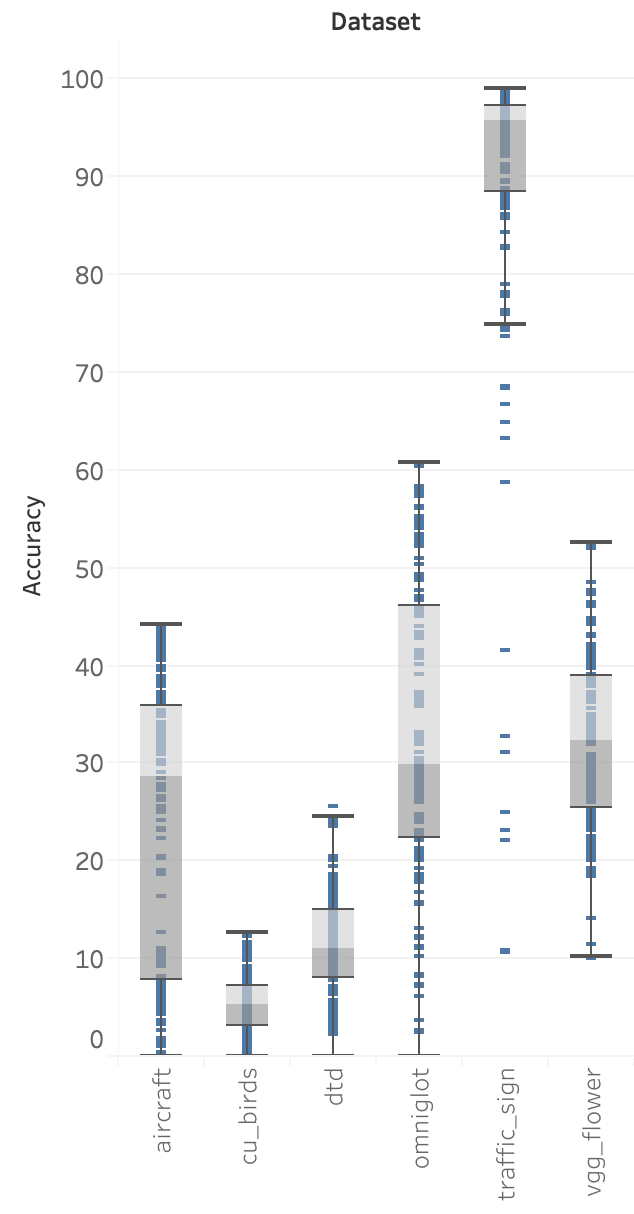
\includegraphics[width=0.8\linewidth]{imgs/boxplot-accuracies.png}
%   \caption{Boxplot of early-stop accuracy values for a subset of the meta-dataset.}
%   \label{fig:appA:boxplot}
% \end{subfigure}%
% \begin{subfigure}{.5\textwidth}
%   \centering
%       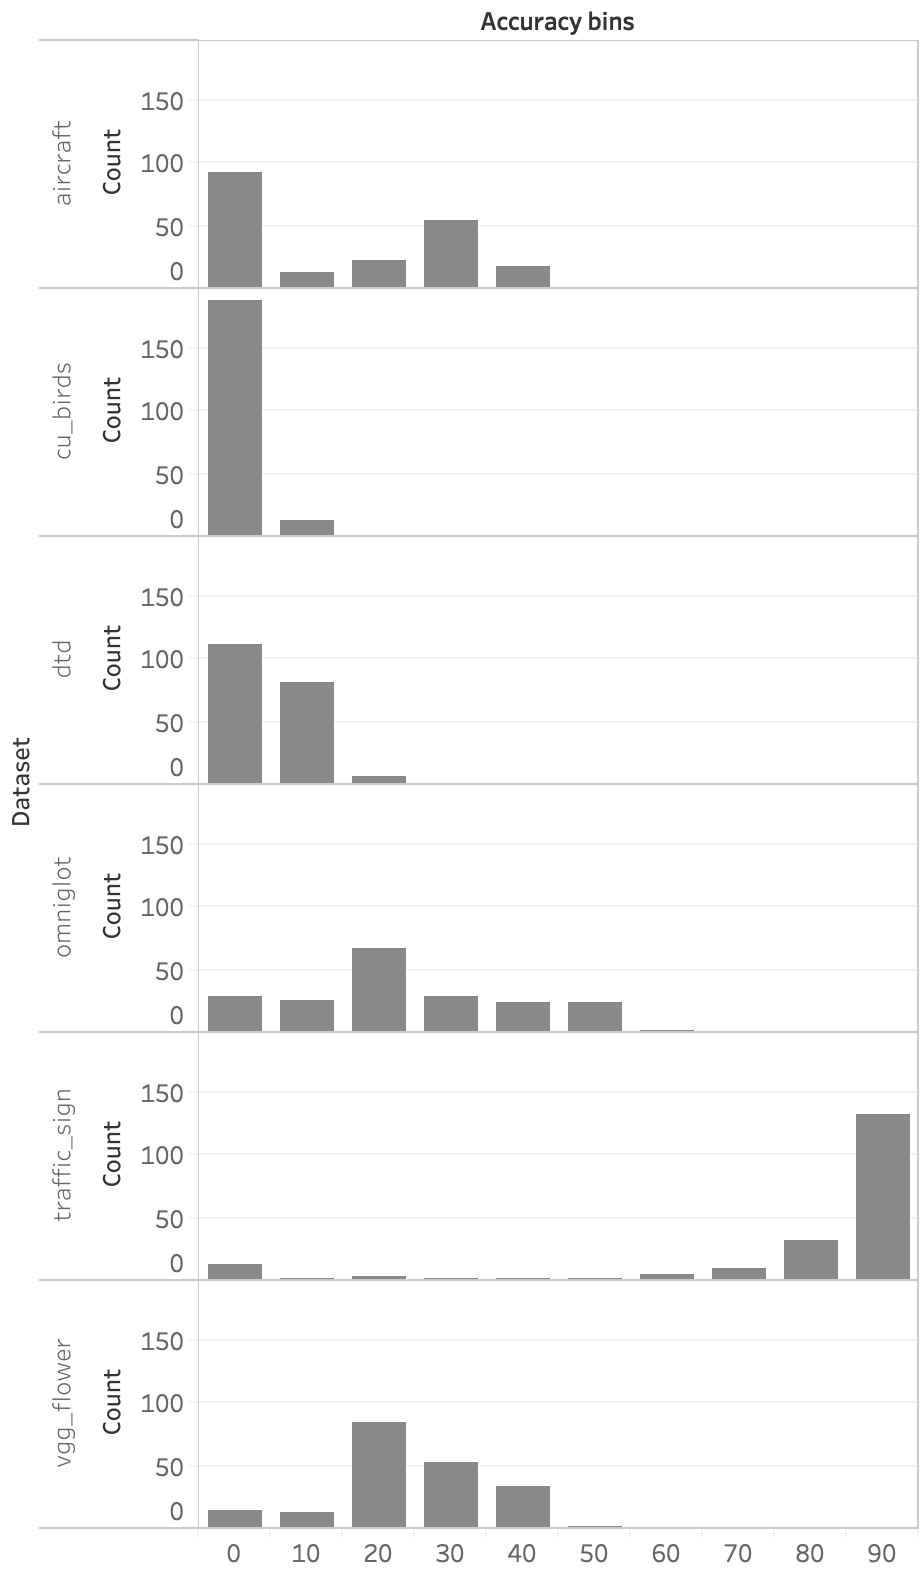
\includegraphics[width=0.9\linewidth]{imgs/histogram-accuracies.png}
%   \caption{Histogram of accuracy values for a subset of the meta-dataset}
%   \label{fig:appA:histogram}
% \end{subfigure}
% \caption{Different visualizations of the early-stop accuracy values obtained in a short deep meta-reinforcement learning trial.}
% \label{fig:appA:trialstats}
% \end{figure}


% \begin{figure}[ht]
%   \centering
%       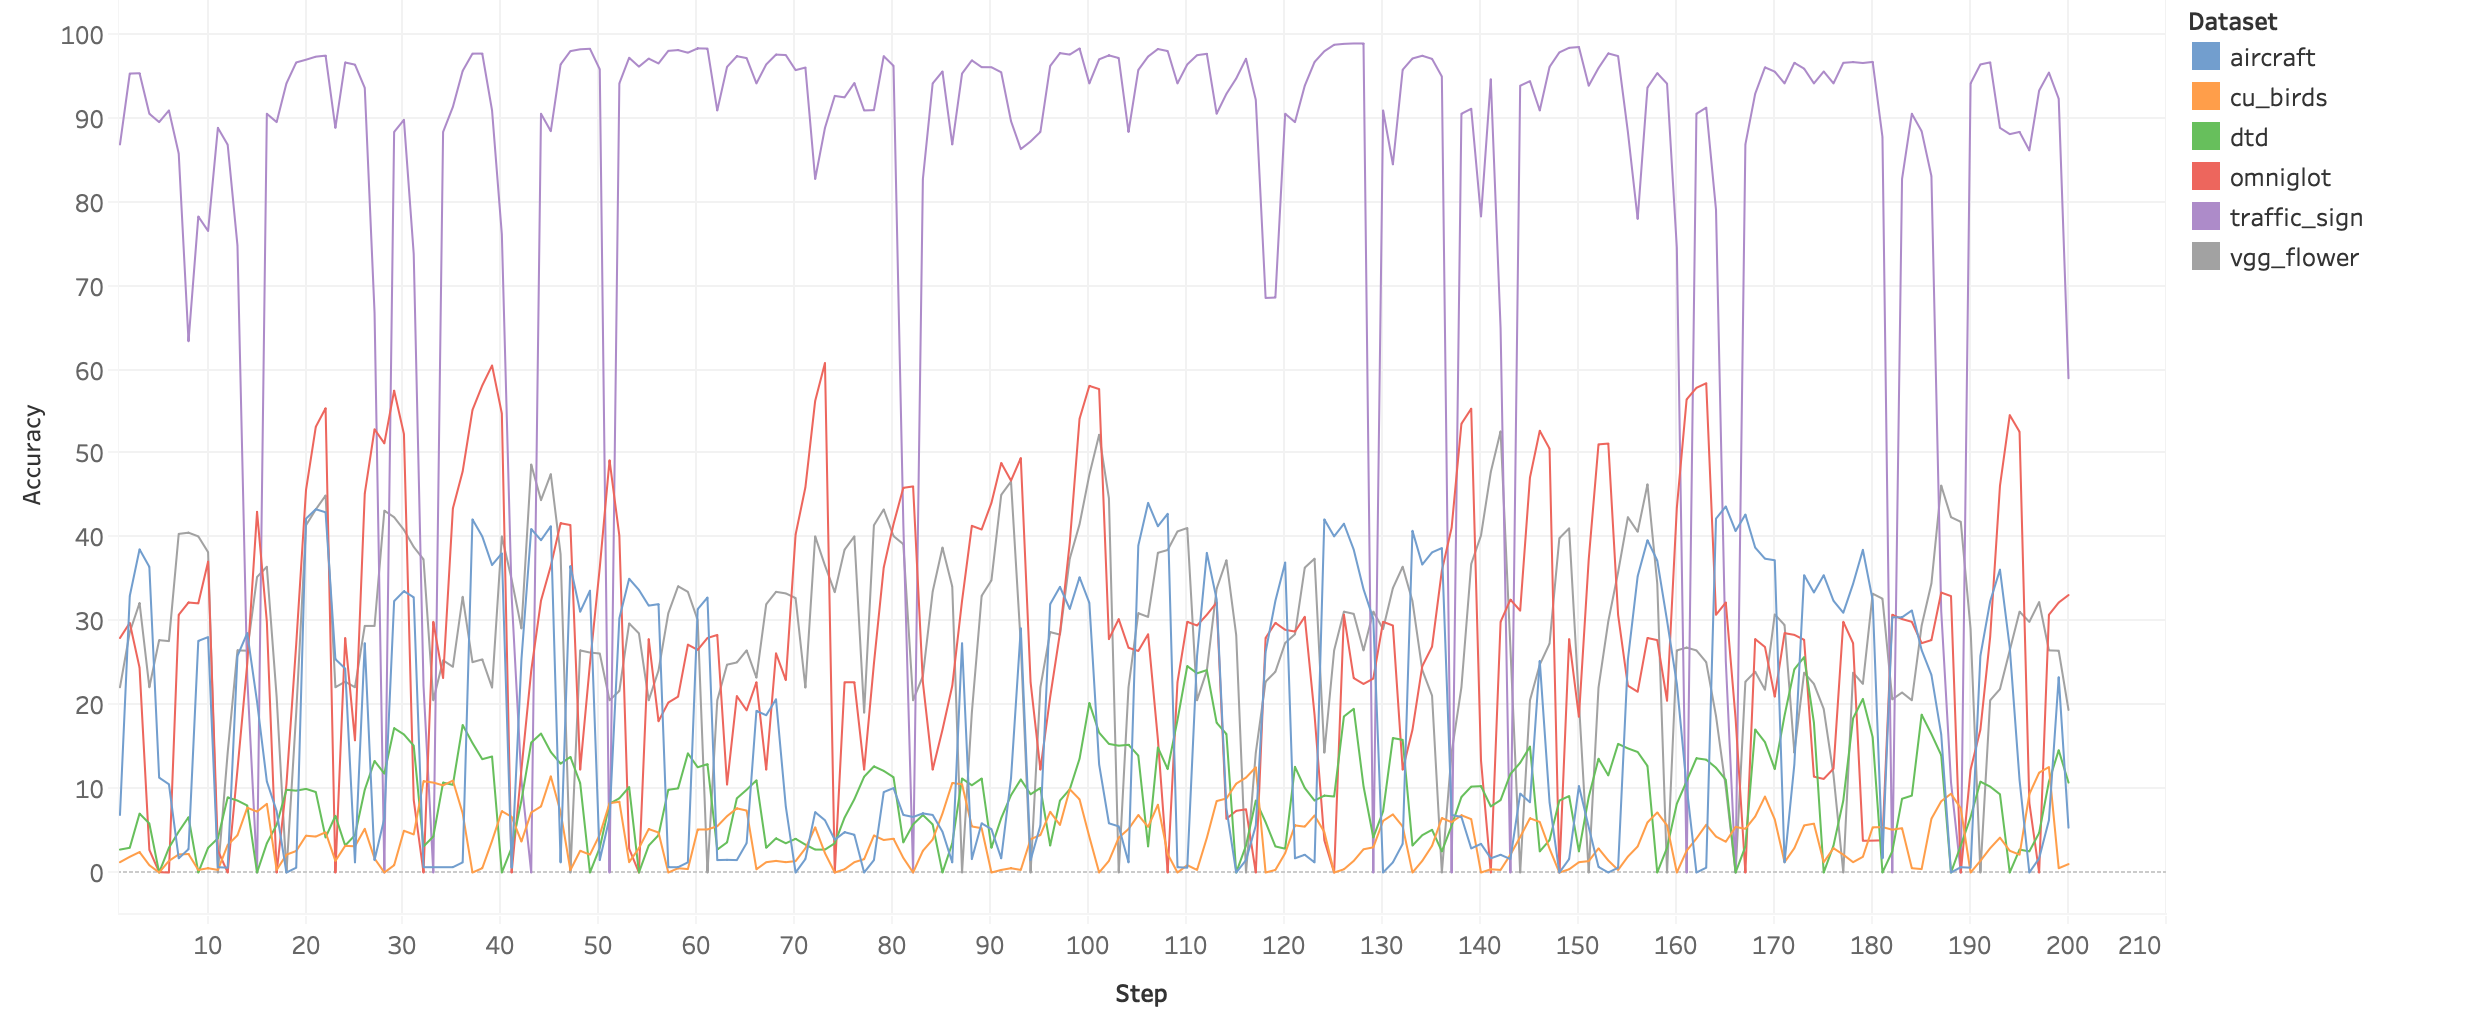
\includegraphics[width=\linewidth]{imgs/all-accuracies.png}
%   \caption{Evolution of early-stop accuracy values for a short deep meta-reinforcement learning trial.}
%   \label{fig:appA:evolution}
% \end{figure}

% This simple exploratory analysis\footnote{A more elaborated analysis would end up in biasing the Neural Architecture Search we aim for, since it would be possible to feed the agent with previous knowledge of the tasks.} suggests three types of datasets: a ``trivial" dataset with high accuracy values with simple networks (\textit{traffic\_sign}), two ``hard" datasets with low accuracy values (all values below 30\%: \textit{dtd} and \textit{cu\_birds}), and three ``medium" datasets with more diversity of accuracy values (median around 30\% and broader interquartile range: \textit{aircraft}, \textit{omniglot}, \textit{vgg\_flower}). On the other hand, for the running times, we can observe that \textit{aircraft} and \textit{cu\_birds} result in expensive experiments, whilst the other 4 are more feasible to complete with our limited computational resources. 

% Considering the computation time, and the hardness of the classification tasks we defined the sampling presented in section~\ref{sec:methodology:rl:environments}, where we have preferred the least-expensive datasets for training.


%%%%%%%%%%%%%%%%%%%%%%%%%%%%%%

\section{Selection of the datasets}\label{app:datasets}

The deep meta-reinforcement learning framework that we implement requires a set of environments associated to image classification tasks. In order to design these environments, we rely on the meta-dataset~\citep{MetaDataset}, a collection of 10 datasets with a concrete sampling procedure designed for meta-learning in few-shot learning image classification. In our setting, the datasets are intended for standard image classification, thus we redefine the sampling strategy. Our interest is in using small but yet challenging datasets that allow us to save computational resources without making the Neural Architecture Search (NAS) trivial.

In Table~\ref{tab:appA:metadataset} the original datasets in the collection are listed. We select the ones that are smaller than CIFAR-10 (60K observations), which is the reference for NAS. The datasets satisfying the criterion are \textit{aircraft}, \textit{cu\_birds}, \textit{dtd}, \textit{omniglot}, \textit{traffic\_sign} and \textit{vgg\_flower}. We want to evaluate the hardness of these six datasets to define a sampling procedure from the collection, and thus we perform a short and individual deep meta-reinforcement learning trial with $t_{max}=200$ for each dataset. Since at the beginning of the trial the agent does not develop any significant knowledge, its sampling of architectures is random. In Figure~\ref{fig:appA:trialstats} the boxplot and barplot of the obtained accuracy values are presented, and in Table~\ref{tab:appA:times} the running time per experiment is shown. 


A simple exploratory analysis suggests three types of datasets: a ``trivial" dataset with high accuracy values with simple networks (\textit{traffic\_sign}), two ``hard" datasets with low accuracy values (all values below 30\%: \textit{dtd} and \textit{cu\_birds}), and three ``medium" datasets with more diversity of accuracy values (median around 30\% and broader interquartile range: \textit{aircraft}, \textit{omniglot}, \textit{vgg\_flower}). On the other hand, for the running times, we can observe that \textit{aircraft} and \textit{cu\_birds} result in the most expensive runs. Considering the computation time, and the hardness of the classification tasks, we defined the sampling presented in Table~\ref{tab:methodology:environments:datasets}. Our training datasets have different levels of hardness and reported the least costly runs.

\begin{table}[ht]
\centering
\begin{tabular}{cccc}
\hline
Dataset ID    & Dataset name                              & N classes & N observations \\ \hline
aircraft      & FGVC-Aircraft                             & 100       & 10000          \\
cu\_birds     & CUB-200-2011                              & 200       & 11788          \\
dtd           & Describable Textures                      & 47        & 5640           \\
fungi         & FGVCx Fungi                               & 1394      & 89760          \\
ilsvrc\_2012  & ImageNet                                  & 1000      & 1280764        \\
mscoco        & Common Objects in Context                 & 80        & 330000         \\
omniglot      & Omniglot                                  & 1623      & 32460          \\
quickdraw     & Quick, Draw!                              & 345       & 50426266       \\
traffic\_sign & German Traffic Sign Recognition Benchmark & 43        & 39209          \\
vgg\_flower   & VGG Flower                                & 102       & 8189           \\ \hline
\end{tabular}
\caption{The original meta-dataset~\citep{MetaDataset} with the number of classes and observations after conversion with the official source code.}
\label{tab:appA:metadataset}
\end{table}



\begin{table}[ht]
\centering
\begin{tabular}{cc}
\hline
Dataset ID    & Time   \\ \hline
aircraft      & 9h49m  \\
cu\_birds     & 16h20m \\
dtd           & 5h38m  \\
omniglot      & 3h38m  \\
traffic\_sign & 4h33m  \\
vgg\_flower   & 4h56m  \\ \hline
\end{tabular}
\caption{Running times of a deep meta-RL trial with $t_{max}=200$, used to study the hardness and cost of each dataset.}
\label{tab:appA:times}
\end{table}

\begin{figure}[ht]
\centering
\begin{subfigure}{.5\textwidth}
  \centering
      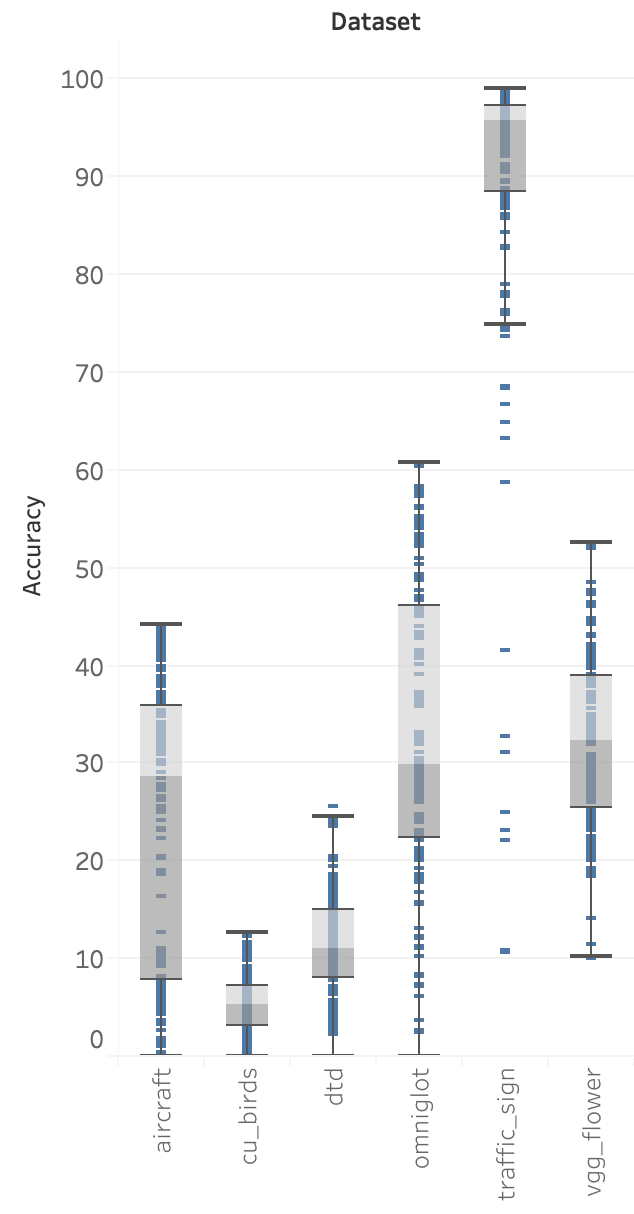
\includegraphics[width=0.8\linewidth]{imgs/boxplot-accuracies.png}
  \caption{}
  \label{fig:appA:boxplot}
\end{subfigure}%
\begin{subfigure}{.5\textwidth}
  \centering
      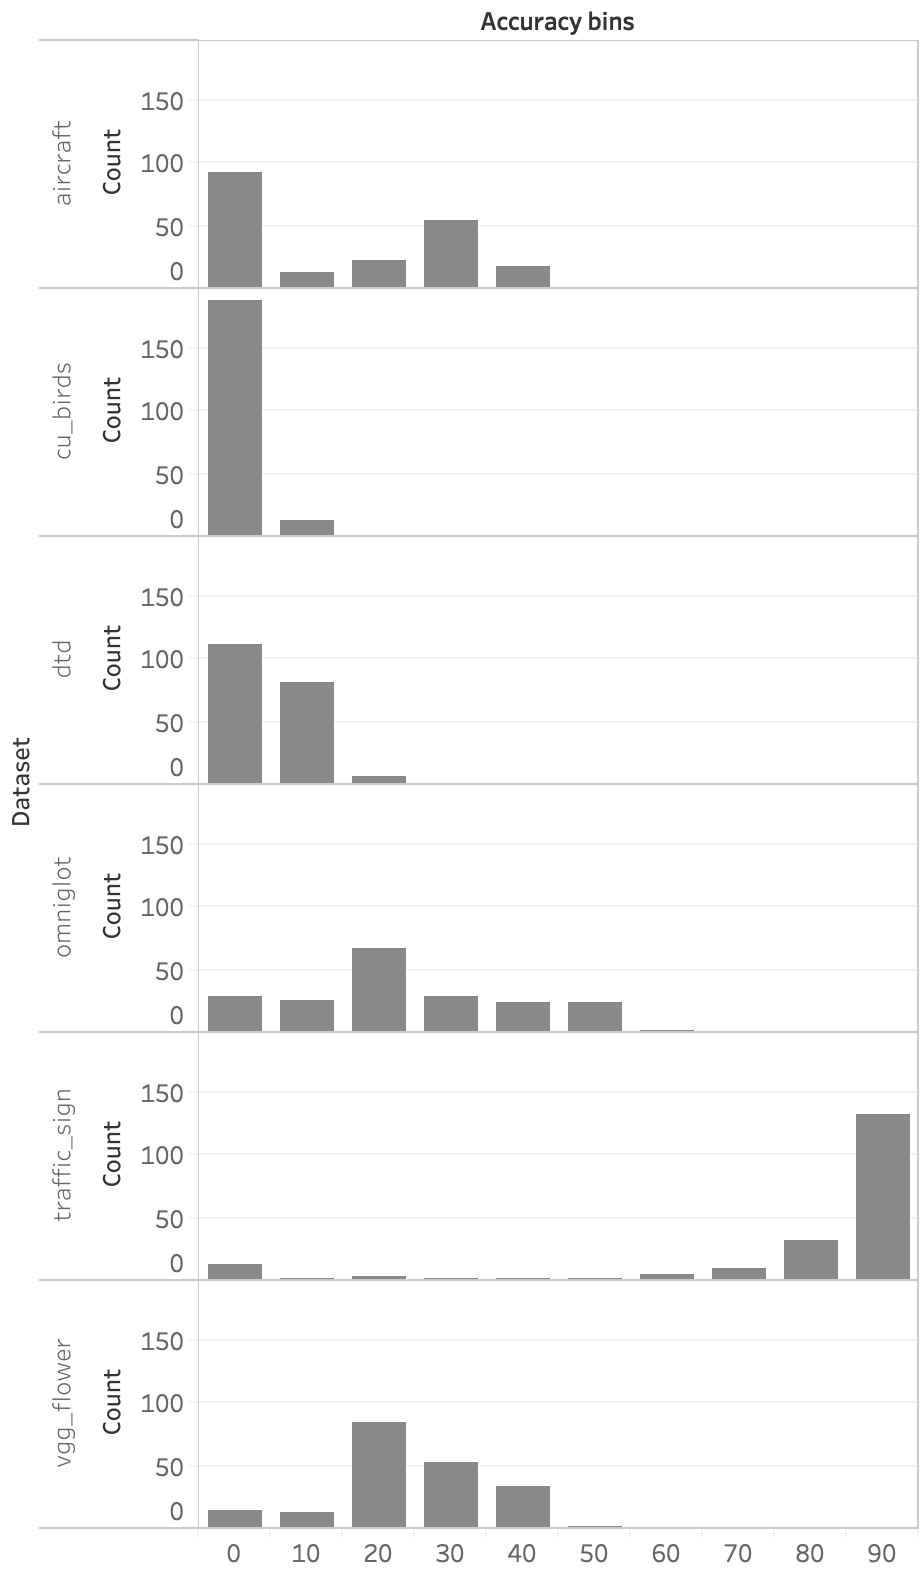
\includegraphics[width=0.9\linewidth]{imgs/histogram-accuracies.png}
  \caption{}
  \label{fig:appA:histogram}
\end{subfigure}
\caption{Different visualizations of the early-stop accuracy values obtained to study the hardness of the datasets.}
\label{fig:appA:trialstats}
\end{figure}




% \appendix
\section{Networks designed by the agent during training and evaluation}\label{app:networks}

Here we show the best architectures designed by the agent in the three experiments. Figure~\ref{fig:app:networks:training} shows the best architecture per datasets during training (\textit{omniglot}, \textit{vgg\_flower}, and \textit{dtd}). Figure~\ref{fig:app:networks:aircraft} and~\ref{fig:app:networks:cubirds} show the best two architectures during evaluation for \textit{aircraft} and \textit{cu\_birds} respectively. Figure~\ref{fig:app:networks:multibranch} shows the best architectures for the multi-branch experiment. For each architecture we report the early-stop accuracy obtained.

%%%%%%%%%%% Training architectures
\begin{figure}[ht]
\centering
\begin{subfigure}{.33\textwidth}
\begin{center}
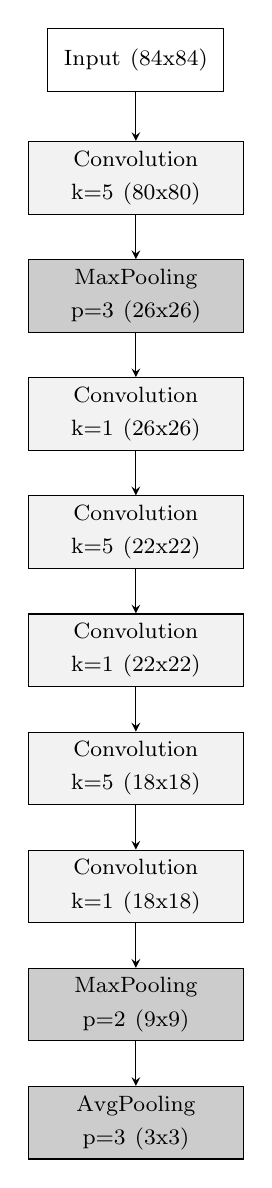
\begin{tikzpicture}

% definitions
\tikzstyle{input} = [rectangle, minimum width=2cm, minimum height=0.8cm, text centered, draw=black, fill=gray!0, text width=2cm]


\tikzstyle{convolution} = [rectangle, minimum width=2cm, minimum height=0.8cm, text centered, draw=black, fill=gray!10, text width=2.5cm]

\tikzstyle{maxpool} = [rectangle, minimum width=2cm, minimum height=0.8cm, text centered, draw=black, fill=gray!40, text width=2.5cm]

\tikzstyle{avgpool} = [rectangle, minimum width=2cm, minimum height=0.8cm, text centered, draw=black, fill=gray!40, text width=2.5cm]

\tikzstyle{concat} = [rectangle, minimum width=2cm, minimum height=0.8cm, text centered, draw=black, fill=gray!80, text width=2.5cm]

\tikzstyle{arrow} = [->,>=stealth]

% the graph
\node (l0) [input] at (0,0) {\footnotesize Input (84x84)};

\node (l1) [convolution, below of=l0, yshift=-0.5cm] {\footnotesize Convolution k=5 (80x80)};

\node (l2) [maxpool, below of=l1, yshift=-0.5cm] {\footnotesize MaxPooling p=3 (26x26)};

\node (l3) [convolution, below of=l2, yshift=-0.5cm] {\footnotesize Convolution k=1 (26x26)};

\node (l4) [convolution, below of=l3, yshift=-0.5cm] {\footnotesize Convolution k=5 (22x22)};

\node (l5) [convolution, below of=l4, yshift=-0.5cm] {\footnotesize Convolution k=1 (22x22)};

\node (l6) [convolution, below of=l5, yshift=-0.5cm] {\footnotesize Convolution k=5 (18x18)};

\node (l7) [convolution, below of=l6, yshift=-0.5cm] {\footnotesize Convolution k=1 (18x18)};

\node (l8) [maxpool, below of=l7, yshift=-0.5cm] {\footnotesize MaxPooling p=2 (9x9)};

\node (l9) [avgpool, below of=l8, yshift=-0.5cm] {\footnotesize AvgPooling p=3 (3x3)};


\draw [arrow] (l0) -- (l1);
\draw [arrow] (l1) -- (l2);
\draw [arrow] (l2) -- (l3);
\draw [arrow] (l3) -- (l4);
\draw [arrow] (l4) -- (l5);
\draw [arrow] (l5) -- (l6);
\draw [arrow] (l6) -- (l7);
\draw [arrow] (l7) -- (l8);
\draw [arrow] (l8) -- (l9);

\end{tikzpicture}
\caption{}
\label{fig:app:networks:training:omniglot}
\end{center}
\end{subfigure}%
\begin{subfigure}{.33\textwidth}
\smallskip
\smallskip
\smallskip
\smallskip
\smallskip
\smallskip
\smallskip
\smallskip
\smallskip
\smallskip
\smallskip
\smallskip
\smallskip
\smallskip
\smallskip
\smallskip
\smallskip
\smallskip
\smallskip
\smallskip
\smallskip
\begin{center}
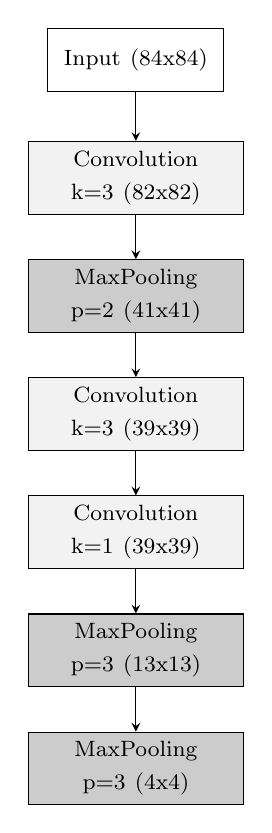
\begin{tikzpicture}

% definitions
\tikzstyle{input} = [rectangle, minimum width=2cm, minimum height=0.8cm, text centered, draw=black, fill=gray!0, text width=2cm]


\tikzstyle{convolution} = [rectangle, minimum width=2cm, minimum height=0.8cm, text centered, draw=black, fill=gray!10, text width=2.5cm]

\tikzstyle{maxpool} = [rectangle, minimum width=2cm, minimum height=0.8cm, text centered, draw=black, fill=gray!40, text width=2.5cm]

\tikzstyle{avgpool} = [rectangle, minimum width=2cm, minimum height=0.8cm, text centered, draw=black, fill=gray!40, text width=2.5cm]

\tikzstyle{concat} = [rectangle, minimum width=2cm, minimum height=0.8cm, text centered, draw=black, fill=gray!80, text width=2.5cm]

\tikzstyle{arrow} = [->,>=stealth]

% the graph
\node (l0) [input] at (0,0) {\footnotesize Input (84x84)};

\node (l1) [convolution, below of=l0, yshift=-0.5cm] {\footnotesize Convolution k=3 (82x82)};

\node (l2) [maxpool, below of=l1, yshift=-0.5cm] {\footnotesize MaxPooling p=2 (41x41)};

\node (l3) [convolution, below of=l2, yshift=-0.5cm] {\footnotesize Convolution k=3 (39x39)};

\node (l4) [convolution, below of=l3, yshift=-0.5cm] {\footnotesize Convolution k=1 (39x39)};

\node (l5) [maxpool, below of=l4, yshift=-0.5cm] {\footnotesize MaxPooling p=3 (13x13)};


\node (l6) [maxpool, below of=l5, yshift=-0.5cm] {\footnotesize MaxPooling p=3 (4x4)};

\draw [arrow] (l0) -- (l1);
\draw [arrow] (l1) -- (l2);
\draw [arrow] (l2) -- (l3);
\draw [arrow] (l3) -- (l4);
\draw [arrow] (l4) -- (l5);
\draw [arrow] (l5) -- (l6);

\end{tikzpicture}
\small
\smallskip
\smallskip
\smallskip
\smallskip
\smallskip
\smallskip
\smallskip
\smallskip
\smallskip
\smallskip
\smallskip
\smallskip
\smallskip
\smallskip
\smallskip
\smallskip
\smallskip
\smallskip
\smallskip
\smallskip
\smallskip
\smallskip
\caption{}
\label{fig:app:networks:training:vggflower}
\end{center}
\end{subfigure}%
\begin{subfigure}{.33\textwidth}
\smallskip
\smallskip
\smallskip
\smallskip
\smallskip
\smallskip
\smallskip
\smallskip
\smallskip
\smallskip
\smallskip
\smallskip
\smallskip
\smallskip
\begin{center}
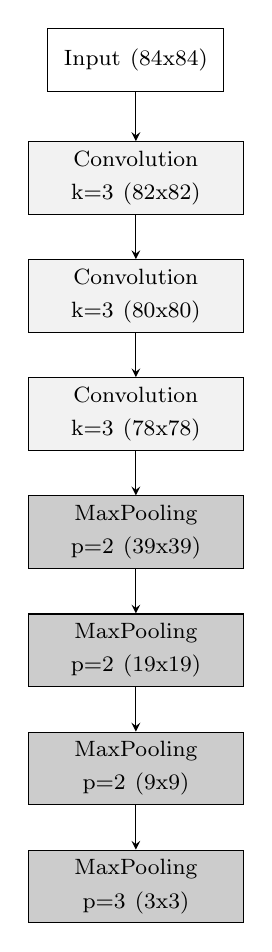
\begin{tikzpicture}

% definitions
\tikzstyle{input} = [rectangle, minimum width=2cm, minimum height=0.8cm, text centered, draw=black, fill=gray!0, text width=2cm]


\tikzstyle{convolution} = [rectangle, minimum width=2cm, minimum height=0.8cm, text centered, draw=black, fill=gray!10, text width=2.5cm]

\tikzstyle{maxpool} = [rectangle, minimum width=2cm, minimum height=0.8cm, text centered, draw=black, fill=gray!40, text width=2.5cm]

\tikzstyle{avgpool} = [rectangle, minimum width=2cm, minimum height=0.8cm, text centered, draw=black, fill=gray!40, text width=2.5cm]

\tikzstyle{concat} = [rectangle, minimum width=2cm, minimum height=0.8cm, text centered, draw=black, fill=gray!80, text width=2.5cm]

\tikzstyle{arrow} = [->,>=stealth]

% the graph
\node (l0) [input] at (0,0) {\footnotesize Input (84x84)};

\node (l1) [convolution, below of=l0, yshift=-0.5cm] {\footnotesize Convolution k=3 (82x82)};

\node (l2) [convolution, below of=l1, yshift=-0.5cm] {\footnotesize Convolution k=3 (80x80)};

\node (l3) [convolution, below of=l2, yshift=-0.5cm] {\footnotesize Convolution k=3 (78x78)};

\node (l4) [maxpool, below of=l3, yshift=-0.5cm] {\footnotesize MaxPooling p=2 (39x39)};

\node (l5) [maxpool, below of=l4, yshift=-0.5cm] {\footnotesize MaxPooling p=2 (19x19)};

\node (l6) [maxpool, below of=l5, yshift=-0.5cm] {\footnotesize MaxPooling p=2 (9x9)};

\node (l7) [maxpool, below of=l6, yshift=-0.5cm] {\footnotesize MaxPooling p=3 (3x3)};


\draw [arrow] (l0) -- (l1);
\draw [arrow] (l1) -- (l2);
\draw [arrow] (l2) -- (l3);
\draw [arrow] (l3) -- (l4);
\draw [arrow] (l4) -- (l5);
\draw [arrow] (l5) -- (l6);
\draw [arrow] (l6) -- (l7);

\end{tikzpicture}
\smallskip
\smallskip
\smallskip
\smallskip
\smallskip
\smallskip
\smallskip
\smallskip
\smallskip
\smallskip
\smallskip
\smallskip
\smallskip
\smallskip
\caption{}
\label{fig:app:networks:training:dtd}
\end{center}
\end{subfigure}
\caption{Best architectures designed for the training datasets. (a) The best architecture for \textit{omniglot}, with early-stop accuracy of 67.11. (b) The best architecture for \textit{vgg\_flower}, with early-stop accuracy of 55.75. (c) The best architecture for \textit{dtd}, with early-stop accuracy of 29.32}
\label{fig:app:networks:training}
\vspace{-0.5cm}
\end{figure}


%%%%%%%%%%%% AIRCRAFT
\begin{figure}[ht]
\centering
\begin{subfigure}{.40\textwidth}
\smallskip
\smallskip
\smallskip
\smallskip
\smallskip
\smallskip
\smallskip
\begin{center}
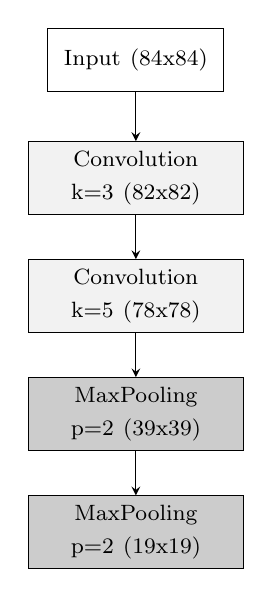
\begin{tikzpicture}

% definitions
\tikzstyle{input} = [rectangle, minimum width=2cm, minimum height=0.8cm, text centered, draw=black, fill=gray!0, text width=2cm]


\tikzstyle{convolution} = [rectangle, minimum width=2cm, minimum height=0.8cm, text centered, draw=black, fill=gray!10, text width=2.5cm]

\tikzstyle{maxpool} = [rectangle, minimum width=2cm, minimum height=0.8cm, text centered, draw=black, fill=gray!40, text width=2.5cm]

\tikzstyle{avgpool} = [rectangle, minimum width=2cm, minimum height=0.8cm, text centered, draw=black, fill=gray!40, text width=2.5cm]

\tikzstyle{concat} = [rectangle, minimum width=2cm, minimum height=0.8cm, text centered, draw=black, fill=gray!80, text width=2.5cm]

\tikzstyle{arrow} = [->,>=stealth]

% the graph
\node (l0) [input] at (0,0) {\footnotesize Input (84x84)};

\node (l1) [convolution, below of=l0, yshift=-0.5cm] {\footnotesize Convolution k=3 (82x82)};

\node (l2) [convolution, below of=l1, yshift=-0.5cm] {\footnotesize Convolution k=5 (78x78)};

\node (l3) [maxpool, below of=l2, yshift=-0.5cm] {\footnotesize MaxPooling p=2 (39x39)};

\node (l4) [maxpool, below of=l3, yshift=-0.5cm] {\footnotesize MaxPooling p=2 (19x19)};


\draw [arrow] (l0) -- (l1);
\draw [arrow] (l1) -- (l2);
\draw [arrow] (l2) -- (l3);
\draw [arrow] (l3) -- (l4);

\end{tikzpicture}
\smallskip
\smallskip
\smallskip
\smallskip
\smallskip
\smallskip
\smallskip
\caption{}
\label{fig:app:networks:aircraft:a}
\end{center}
\end{subfigure}%
\begin{subfigure}{.40\textwidth}
\begin{center}
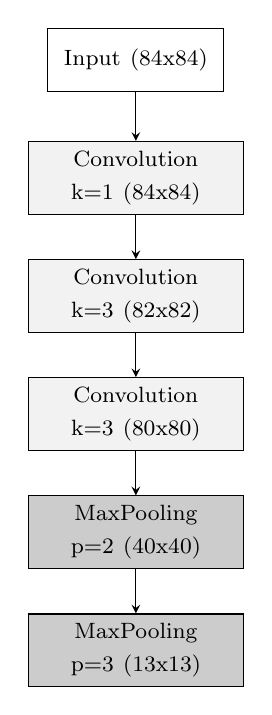
\begin{tikzpicture}

% definitions
\tikzstyle{input} = [rectangle, minimum width=2cm, minimum height=0.8cm, text centered, draw=black, fill=gray!0, text width=2cm]


\tikzstyle{convolution} = [rectangle, minimum width=2cm, minimum height=0.8cm, text centered, draw=black, fill=gray!10, text width=2.5cm]

\tikzstyle{maxpool} = [rectangle, minimum width=2cm, minimum height=0.8cm, text centered, draw=black, fill=gray!40, text width=2.5cm]

\tikzstyle{avgpool} = [rectangle, minimum width=2cm, minimum height=0.8cm, text centered, draw=black, fill=gray!40, text width=2.5cm]

\tikzstyle{concat} = [rectangle, minimum width=2cm, minimum height=0.8cm, text centered, draw=black, fill=gray!80, text width=2.5cm]

\tikzstyle{arrow} = [->,>=stealth]

% the graph
\node (l0) [input] at (0,0) {\footnotesize Input (84x84)};

\node (l1) [convolution, below of=l0, yshift=-0.5cm] {\footnotesize Convolution k=1 (84x84)};

\node (l2) [convolution, below of=l1, yshift=-0.5cm] {\footnotesize Convolution k=3 (82x82)};

\node (l3) [convolution, below of=l2, yshift=-0.5cm] {\footnotesize Convolution k=3 (80x80)};

\node (l4) [maxpool, below of=l3, yshift=-0.5cm] {\footnotesize MaxPooling p=2 (40x40)};

\node (l5) [maxpool, below of=l4, yshift=-0.5cm] {\footnotesize MaxPooling p=3 (13x13)};


\draw [arrow] (l0) -- (l1);
\draw [arrow] (l1) -- (l2);
\draw [arrow] (l2) -- (l3);
\draw [arrow] (l3) -- (l4);
\draw [arrow] (l4) -- (l5);

\end{tikzpicture}
\small
\caption{}
\label{fig:app:networks:aircraft:b}
\end{center}
\end{subfigure}
\caption{Best architectures designed for \textit{aircraft} during evaluation of the policy. (a) The best architecture with early-stop accuracy of 48.22. (b) The second-best architecture with early-stop accuracy of 47.95}
\label{fig:app:networks:aircraft}
\vspace{-0.5cm}
\end{figure}


%%%%%%%%% CU BIRDS

\begin{figure}[ht]
\centering
\begin{subfigure}{.40\textwidth}
\begin{center}
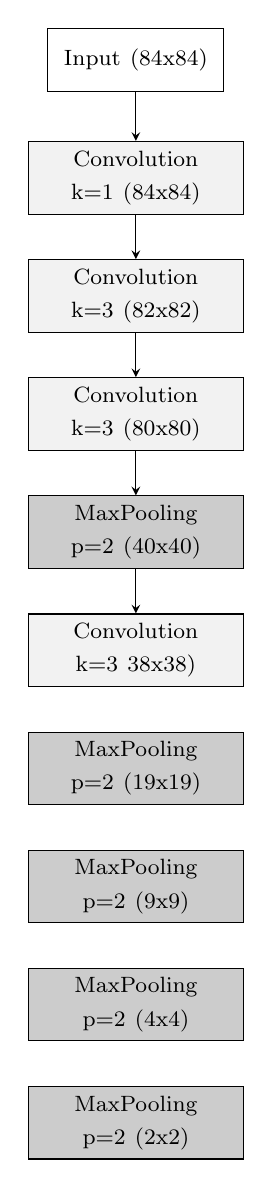
\begin{tikzpicture}

% definitions
\tikzstyle{input} = [rectangle, minimum width=2cm, minimum height=0.8cm, text centered, draw=black, fill=gray!0, text width=2cm]


\tikzstyle{convolution} = [rectangle, minimum width=2cm, minimum height=0.8cm, text centered, draw=black, fill=gray!10, text width=2.5cm]

\tikzstyle{maxpool} = [rectangle, minimum width=2cm, minimum height=0.8cm, text centered, draw=black, fill=gray!40, text width=2.5cm]

\tikzstyle{avgpool} = [rectangle, minimum width=2cm, minimum height=0.8cm, text centered, draw=black, fill=gray!40, text width=2.5cm]

\tikzstyle{concat} = [rectangle, minimum width=2cm, minimum height=0.8cm, text centered, draw=black, fill=gray!80, text width=2.5cm]

\tikzstyle{arrow} = [->,>=stealth]

% the graph
\node (l0) [input] at (0,0) {\footnotesize Input (84x84)};

\node (l1) [convolution, below of=l0, yshift=-0.5cm] {\footnotesize Convolution k=1 (84x84)};

\node (l2) [convolution, below of=l1, yshift=-0.5cm] {\footnotesize Convolution k=3 (82x82)};

\node (l3) [convolution, below of=l2, yshift=-0.5cm] {\footnotesize Convolution k=3 (80x80)};

\node (l4) [maxpool, below of=l3, yshift=-0.5cm] {\footnotesize MaxPooling p=2 (40x40)};

\node (l5) [convolution, below of=l4, yshift=-0.5cm] {\footnotesize Convolution k=3 38x38)};

\node (l6) [maxpool, below of=l5, yshift=-0.5cm] {\footnotesize MaxPooling p=2 (19x19)};

\node (l7) [maxpool, below of=l6, yshift=-0.5cm] {\footnotesize MaxPooling p=2 (9x9)};

\node (l8) [maxpool, below of=l7, yshift=-0.5cm] {\footnotesize MaxPooling p=2 (4x4)};

\node (l9) [maxpool, below of=l8, yshift=-0.5cm] {\footnotesize MaxPooling p=2 (2x2)};

\draw [arrow] (l0) -- (l1);
\draw [arrow] (l1) -- (l2);
\draw [arrow] (l2) -- (l3);
\draw [arrow] (l3) -- (l4);
\draw [arrow] (l4) -- (l5);

\end{tikzpicture}
% \smallskip
% \smallskip
% \smallskip
% \smallskip
% \smallskip
% \smallskip
% \smallskip
% \smallskip
% \smallskip
% \smallskip
% \smallskip
% \smallskip
% \smallskip
% \smallskip
\caption{}
\label{fig:app:networks:cubirds:a}
\end{center}
\end{subfigure}%
\begin{subfigure}{.40\textwidth}
\begin{center}
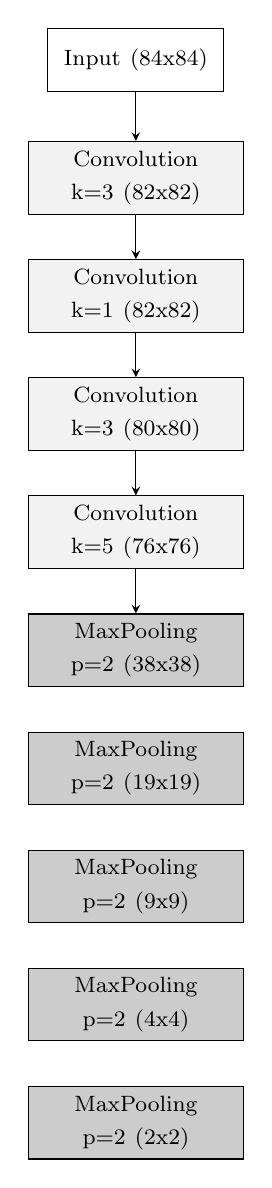
\begin{tikzpicture}

% definitions
\tikzstyle{input} = [rectangle, minimum width=2cm, minimum height=0.8cm, text centered, draw=black, fill=gray!0, text width=2cm]


\tikzstyle{convolution} = [rectangle, minimum width=2cm, minimum height=0.8cm, text centered, draw=black, fill=gray!10, text width=2.5cm]

\tikzstyle{maxpool} = [rectangle, minimum width=2cm, minimum height=0.8cm, text centered, draw=black, fill=gray!40, text width=2.5cm]

\tikzstyle{avgpool} = [rectangle, minimum width=2cm, minimum height=0.8cm, text centered, draw=black, fill=gray!40, text width=2.5cm]

\tikzstyle{concat} = [rectangle, minimum width=2cm, minimum height=0.8cm, text centered, draw=black, fill=gray!80, text width=2.5cm]

\tikzstyle{arrow} = [->,>=stealth]

% the graph
\node (l0) [input] at (0,0) {\footnotesize Input (84x84)};

\node (l1) [convolution, below of=l0, yshift=-0.5cm] {\footnotesize Convolution k=3 (82x82)};

\node (l2) [convolution, below of=l1, yshift=-0.5cm] {\footnotesize Convolution k=1 (82x82)};

\node (l3) [convolution, below of=l2, yshift=-0.5cm] {\footnotesize Convolution k=3 (80x80)};

\node (l4) [convolution, below of=l3, yshift=-0.5cm] {\footnotesize Convolution k=5 (76x76)};

\node (l5) [maxpool, below of=l4, yshift=-0.5cm] {\footnotesize MaxPooling p=2 (38x38)};

\node (l6) [maxpool, below of=l5, yshift=-0.5cm] {\footnotesize MaxPooling p=2 (19x19)};

\node (l7) [maxpool, below of=l6, yshift=-0.5cm] {\footnotesize MaxPooling p=2 (9x9)};

\node (l8) [maxpool, below of=l7, yshift=-0.5cm] {\footnotesize MaxPooling p=2 (4x4)};

\node (l9) [maxpool, below of=l8, yshift=-0.5cm] {\footnotesize MaxPooling p=2 (2x2)};

\draw [arrow] (l0) -- (l1);
\draw [arrow] (l1) -- (l2);
\draw [arrow] (l2) -- (l3);
\draw [arrow] (l3) -- (l4);
\draw [arrow] (l4) -- (l5);

\end{tikzpicture}
\small
\caption{}
\label{fig:app:networks:cubirds:b}
\end{center}
\end{subfigure}
\caption{Best architectures designed for \textit{cu\_birds} during evaluation of the policy. (a) The best architecture with early-stop accuracy of 19.22. (b) The second-best architecture with early-stop accuracy of 19.06}
\label{fig:app:networks:cubirds}
\vspace{-0.5cm}
\end{figure}

%%%%%%%%%%%%%% multibranch

\begin{figure}[ht]
\centering
\begin{subfigure}{.40\textwidth}
\begin{center}
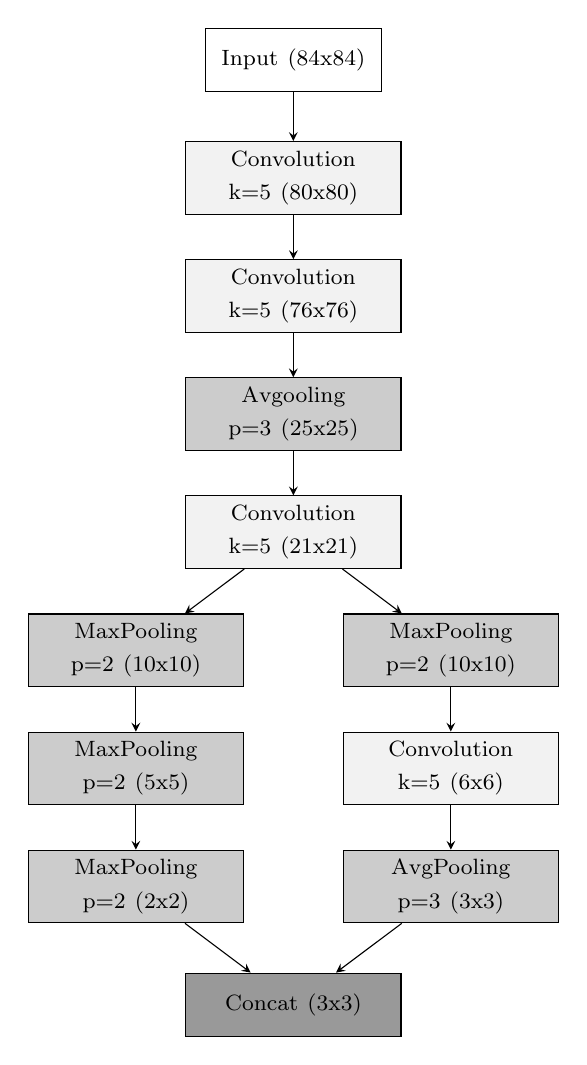
\begin{tikzpicture}

% definitions
\tikzstyle{input} = [rectangle, minimum width=2cm, minimum height=0.8cm, text centered, draw=black, fill=gray!0, text width=2cm]


\tikzstyle{convolution} = [rectangle, minimum width=2cm, minimum height=0.8cm, text centered, draw=black, fill=gray!10, text width=2.5cm]

\tikzstyle{maxpool} = [rectangle, minimum width=2cm, minimum height=0.8cm, text centered, draw=black, fill=gray!40, text width=2.5cm]

\tikzstyle{avgpool} = [rectangle, minimum width=2cm, minimum height=0.8cm, text centered, draw=black, fill=gray!40, text width=2.5cm]

\tikzstyle{concat} = [rectangle, minimum width=2cm, minimum height=0.8cm, text centered, draw=black, fill=gray!80, text width=2.5cm]

\tikzstyle{arrow} = [->,>=stealth]

% the graph
\node (l0) [input] at (0,0) {\footnotesize Input (84x84)};

\node (l1) [convolution, below of=l0, yshift=-0.5cm] {\footnotesize Convolution k=5 (80x80)};

\node (l2) [convolution, below of=l1, yshift=-0.5cm] {\footnotesize Convolution k=5 (76x76)};

\node (l3) [avgpool, below of=l2, yshift=-0.5cm] {\footnotesize Avgooling p=3 (25x25)};

\node (l4) [convolution, below of=l3, yshift=-0.5cm] {\footnotesize Convolution k=5 (21x21)};

\node (l5) [maxpool, below of=l4, yshift=-0.5cm, xshift=-2cm] {\footnotesize MaxPooling p=2 (10x10)};

\node (l6) [maxpool, below of=l4, yshift=-0.5cm, xshift=2cm] {\footnotesize MaxPooling p=2 (10x10)};

\node (l7) [maxpool, below of=l5, yshift=-0.5cm] {\footnotesize MaxPooling p=2 (5x5)};

\node (l8) [convolution, below of=l6, yshift=-0.5cm] {\footnotesize Convolution k=5 (6x6)};

\node (l9) [maxpool, below of=l7, yshift=-0.5cm] {\footnotesize MaxPooling p=2 (2x2)};

\node (l10) [avgpool, below of=l8, yshift=-0.5cm] {\footnotesize AvgPooling p=3 (3x3)};

\node (l11) [concat, below of=l10, yshift=-0.5cm, xshift=-2cm] {\footnotesize Concat (3x3)};


\draw [arrow] (l0) -- (l1);
\draw [arrow] (l1) -- (l2);
\draw [arrow] (l2) -- (l3);
\draw [arrow] (l3) -- (l4);
\draw [arrow] (l4) -- (l5);
\draw [arrow] (l4) -- (l6);
\draw [arrow] (l5) -- (l7);
\draw [arrow] (l6) -- (l8);
\draw [arrow] (l7) -- (l9);
\draw [arrow] (l8) -- (l10);
\draw [arrow] (l9) -- (l11);
\draw [arrow] (l10) -- (l11);

\end{tikzpicture}
\caption{}
\label{fig:app:networks:multibranch:a}
\end{center}
\end{subfigure}%
\begin{subfigure}{.40\textwidth}
\begin{center}
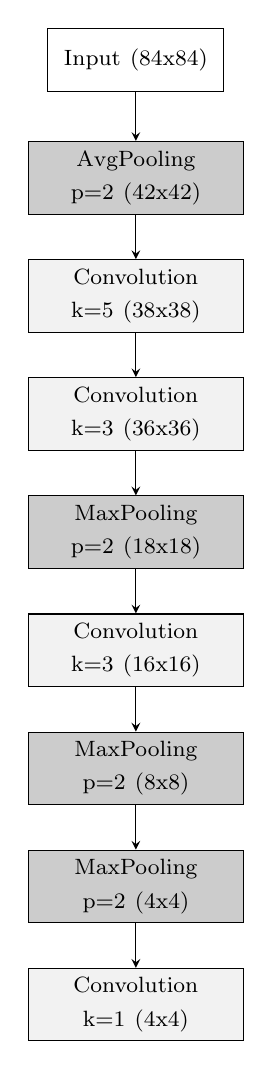
\begin{tikzpicture}

% definitions
\tikzstyle{input} = [rectangle, minimum width=2cm, minimum height=0.8cm, text centered, draw=black, fill=gray!0, text width=2cm]


\tikzstyle{convolution} = [rectangle, minimum width=2cm, minimum height=0.8cm, text centered, draw=black, fill=gray!10, text width=2.5cm]

\tikzstyle{maxpool} = [rectangle, minimum width=2cm, minimum height=0.8cm, text centered, draw=black, fill=gray!40, text width=2.5cm]

\tikzstyle{avgpool} = [rectangle, minimum width=2cm, minimum height=0.8cm, text centered, draw=black, fill=gray!40, text width=2.5cm]

\tikzstyle{concat} = [rectangle, minimum width=2cm, minimum height=0.8cm, text centered, draw=black, fill=gray!80, text width=2.5cm]

\tikzstyle{arrow} = [->,>=stealth]

% the graph
\node (l0) [input] at (0,0) {\footnotesize Input (84x84)};

\node (l1) [avgpool, below of=l0, yshift=-0.5cm] {\footnotesize AvgPooling p=2 (42x42)};

\node (l2) [convolution, below of=l1, yshift=-0.5cm] {\footnotesize Convolution k=5 (38x38)};

\node (l3) [convolution, below of=l2, yshift=-0.5cm] {\footnotesize Convolution k=3 (36x36)};

\node (l4) [maxpool, below of=l3, yshift=-0.5cm] {\footnotesize MaxPooling p=2 (18x18)};

\node (l5) [convolution, below of=l4, yshift=-0.5cm] {\footnotesize Convolution k=3 (16x16)};

\node (l6) [maxpool, below of=l5, yshift=-0.5cm] {\footnotesize MaxPooling p=2 (8x8)};

\node (l7) [maxpool, below of=l6, yshift=-0.5cm] {\footnotesize MaxPooling p=2 (4x4)};

\node (l8) [convolution, below of=l7, yshift=-0.5cm] {\footnotesize Convolution k=1 (4x4)};

\draw [arrow] (l0) -- (l1);
\draw [arrow] (l1) -- (l2);
\draw [arrow] (l2) -- (l3);
\draw [arrow] (l3) -- (l4);
\draw [arrow] (l4) -- (l5);
\draw [arrow] (l5) -- (l6);
\draw [arrow] (l6) -- (l7);
\draw [arrow] (l7) -- (l8);

\end{tikzpicture}
\small
\caption{}
\label{fig:app:networks:multibranch:b}
\end{center}
\end{subfigure}
\caption{Best architectures designed for during the experiment in a multi-branch search space. (a) The best architecture when $\sigma=0.0$, with early-stop accuracy of 66.10. (b) The best architecture when $\sigma=0.1$, with early-stop accuracy of 66.45}
\label{fig:app:networks:multibranch}
\vspace{-0.5cm}
\end{figure}



\end{document}